\chapter{Drone Design and Construction}

A drone is designed and constructed. The goal is to be cost-effective and to source local supplies. It should be note that pre-built drones like the DJI Phantom and Inspire cost significantly more\footnote{Roughly 100\% to 200\% more}.

\section{Drone}

A quadcopter was designed and built to handle all the equipment.

\subsection{Mechanical subsystem design}

The drone will be medium sized, with a payload of 1kg.

\subsubsection{Frame}

There are many materials and configurations for a drone. The configurations include 3, 4, 6, 8 arms or more, with single or contra-rotating propellers on each arm\footnote{Two propellers aligned vertically and spinning opposite to each other for upwards thrust}. \\

Aerial cinematography requires a stiff but less brittle frame to provide a smooth and stable flight. They also need to be large enough to hold the cameras needed for this professional activity. Lastly, the frames should be supportive of tall landing gear \cite{frame}. Due to the larger overall mass, the frame's natural frequency is low, meaning that it provides the same stability as a hand-held weighted gimbal in cinematography. For our application, we'll be using lightweight cameras, which weigh 3 grams each, which means our drone can be lighter.\\

Recreational usage may use 'mini multicopter frames' for flying indoors and outdoors \cite{frame}. They're extremely light, but do not have enough space for other peripherals\footnote{GPS, Raspberry Pis etcetra}.\\

Sports drones are light and fast, but they require high discharge batteries which are not cost effective for our application. Besides, they do not have enough space.\\

A combination of these configurations means that a medium sized quadcopter\footnote{Four propellers} will be suitable. It is not too light or too heavy, and has room for other peripherals.

Materials include carbon-fibre, aluminium and fibreglass and synthetic polymers. The differences between them are not major, except that aluminium is heavier, requires larger motors and induces more vibrations. Carbon-fibre contributes to radio interference\cite{frame}, but is the lightest.

The closest competition before the F450-V2 quadcopter frame was chosen was the ZMR250 Carbon Mini Quad FPV Frame as in Figure \ref{fig:zmr}.

\begin{figure}[H]
\centering
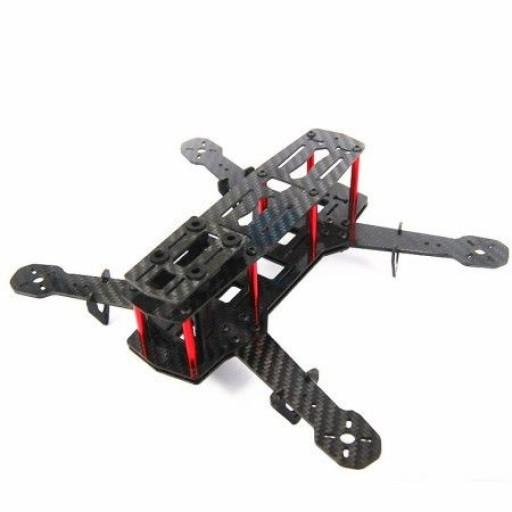
\includegraphics[scale=0.35]{images/zmr250.jpeg}
\caption{ZMR250 Carbon Mini Quad FPV Frame \cite{frobot}}
\label{fig:zmr}
\end{figure}

Both frames have roughly the same price\footnote{500 ZAR}.\\

The ZMR250 has a carbon fibre body making it extremely light (145g), but fell into the class of `mini multicopter` as mentioned earlier. There was not enough space for the other peripherals as well.\\

Therefore due to its local availability and accommodating space, the F450-V2 frame was chosen as in Figure \ref{fig:frame}.

\subsubsection{Landing Gear}

Four lengths of 10mm pine dowels approximately 15mm long were used. They totalled about 10 ZAR. The frame has 5cm legs, but accomodation has to be made for the nadir cameras.

\subsubsection{Motors}

The motors are rated at 920 KV\footnote{KV is a measure of the revolutions per minute when 1 Volt is applied with no load attached to the motor}. This is relatively low compared to the more common racing motors with around 2000 KV (which the ZMR250 frame would use). KV is related to the power output and torque level of a motor. This is determined by the number of turns on the armature and the strength of the magnets.

\subsubsection{Protective enclosure}

The flight controller requires a protective enclosure. A case\cite{3d_case} was 3D printed for the Raspberry Pi as in Figure \ref{fig:fcarpc2}.

\subsection{Electrical subsystem design}
\subsubsection{Batteries}

Multiple 3S1P batteries will be used, since the price cost-point was the cheapest (explain). (insert picture)

\subsubsection{Dual power redundancy}

The flight controller takes in two power source inputs for dual redundancy as in Figure \ref{fig:dual_redundancy}. One of the batteries powers the motors during flight. This also allows the electronics to remain on when swapping out the flight battery.

\begin{figure}[H]
\centering
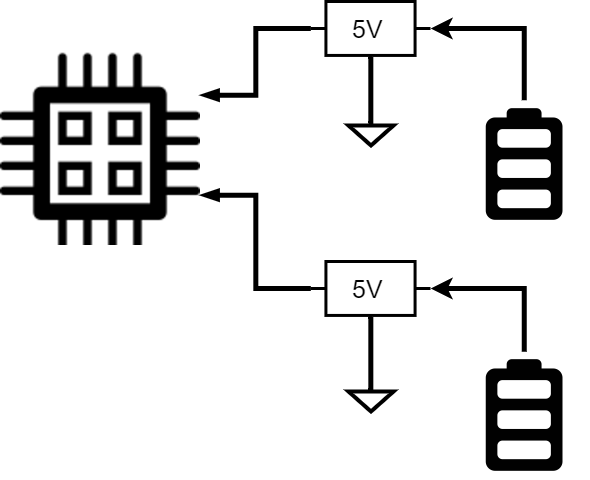
\includegraphics[scale=0.35]{images/dual_redundancy.png}
\caption{Illustrating dual power redundancy}
\label{fig:dual_redundancy}
\end{figure}

\subsubsection{Electronic speed controllers}

The 3-phase motors require speed control. This is achieved by ESCs. Maximum power draw from the motors is

\subsection{Electronic subsystem design}

\subsubsection{Flight controller}
Flight controller is needed to stabilize the airborne vehicle, and set mission waypoints. The Raspberry Pi, Navio2, and camera symbiosis was good since all three together are quite configurable even during flight, compared to other solutions which require hands-on intervention.

\subsection{Communication subsystem design}

2.4 GHz, and 433 MHz is used.

\subsection{Sensor subsystem design}

Barometer, etc, redundancy.

\subsection{Construction process and Integration}

At first, the frame is put together. This gives one a good idea of the actual size from the beginning.

\begin{figure}[H]
\begin{subfigure}{0.5\textwidth}
\centering
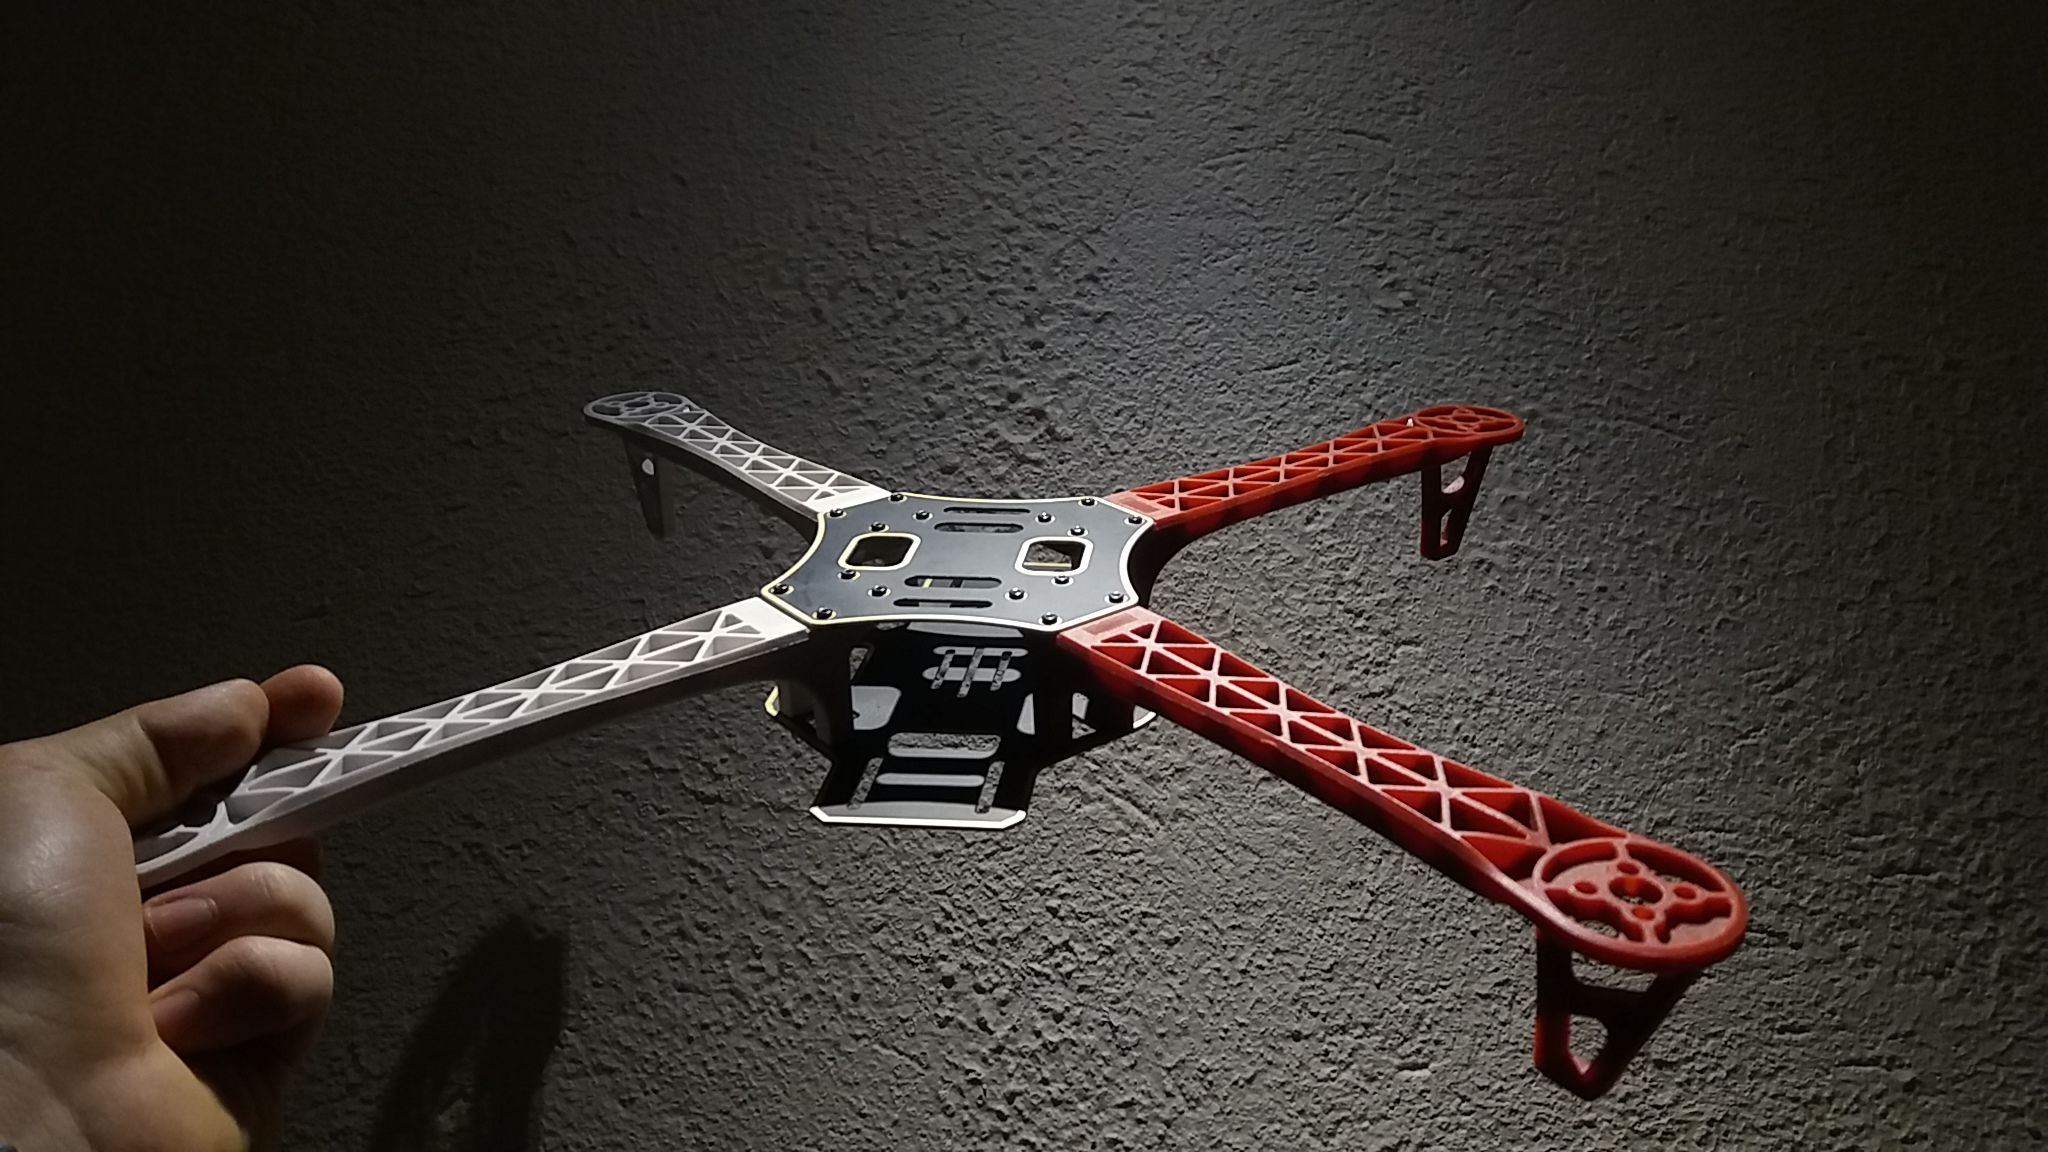
\includegraphics[scale=0.1]{images/drone-build-frame.jpg}
\caption{F450-V2 frame.}
\label{fig:frame}
\end{subfigure}
\begin{subfigure}{0.5\textwidth}
\centering
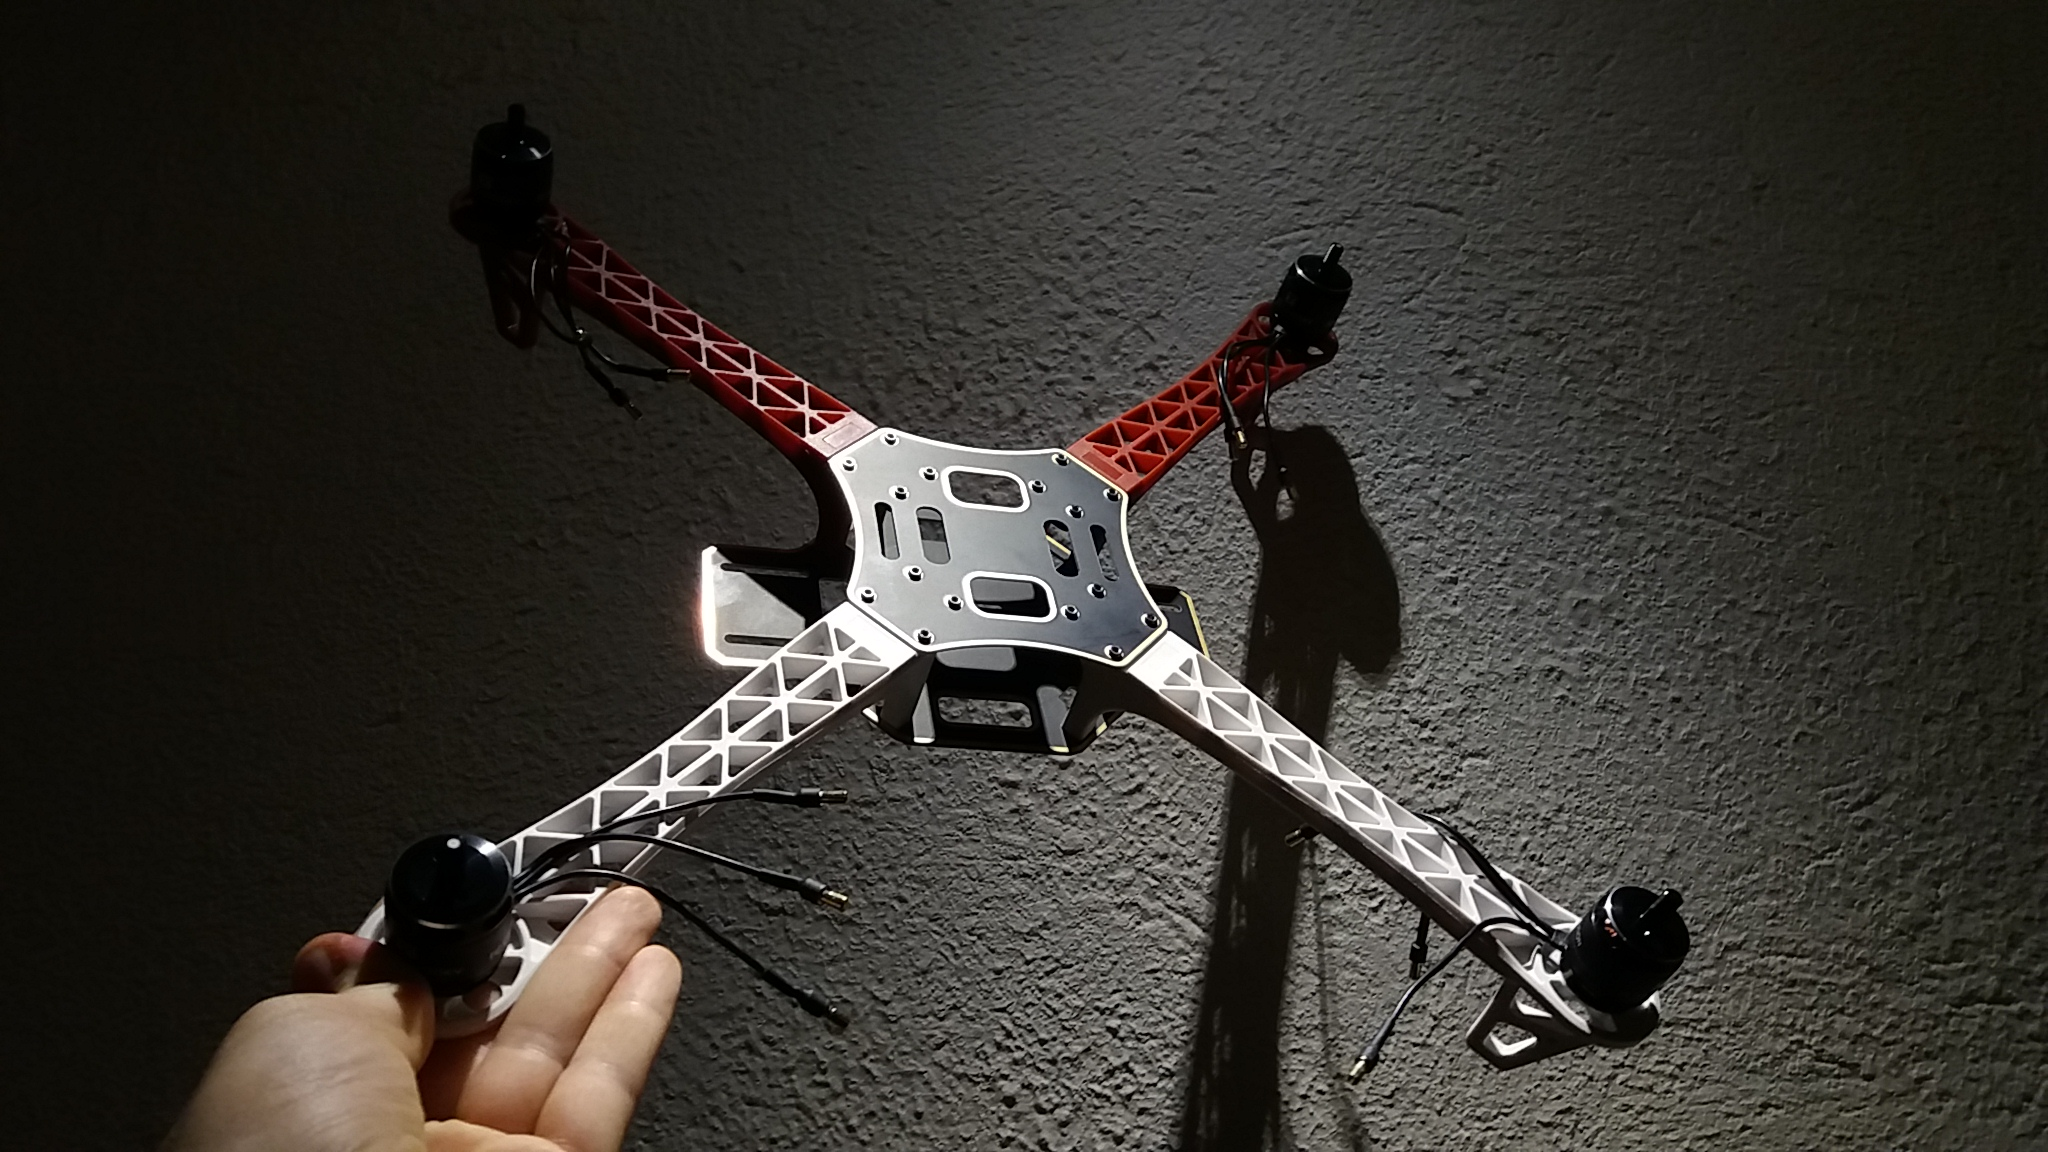
\includegraphics[scale=0.1]{images/drone-build-motors.jpg}
\caption{Adding the 920kv motors.}
\label{fig:motors}
\end{subfigure}
\caption{Frame and motors}
\label{fig:frame_motors}
\end{figure}

The frame is made out of a nylon polymer as in Figure \ref{fig:frame}.\\

\begin{figure}[H]
\begin{subfigure}{0.5\textwidth}
\centering
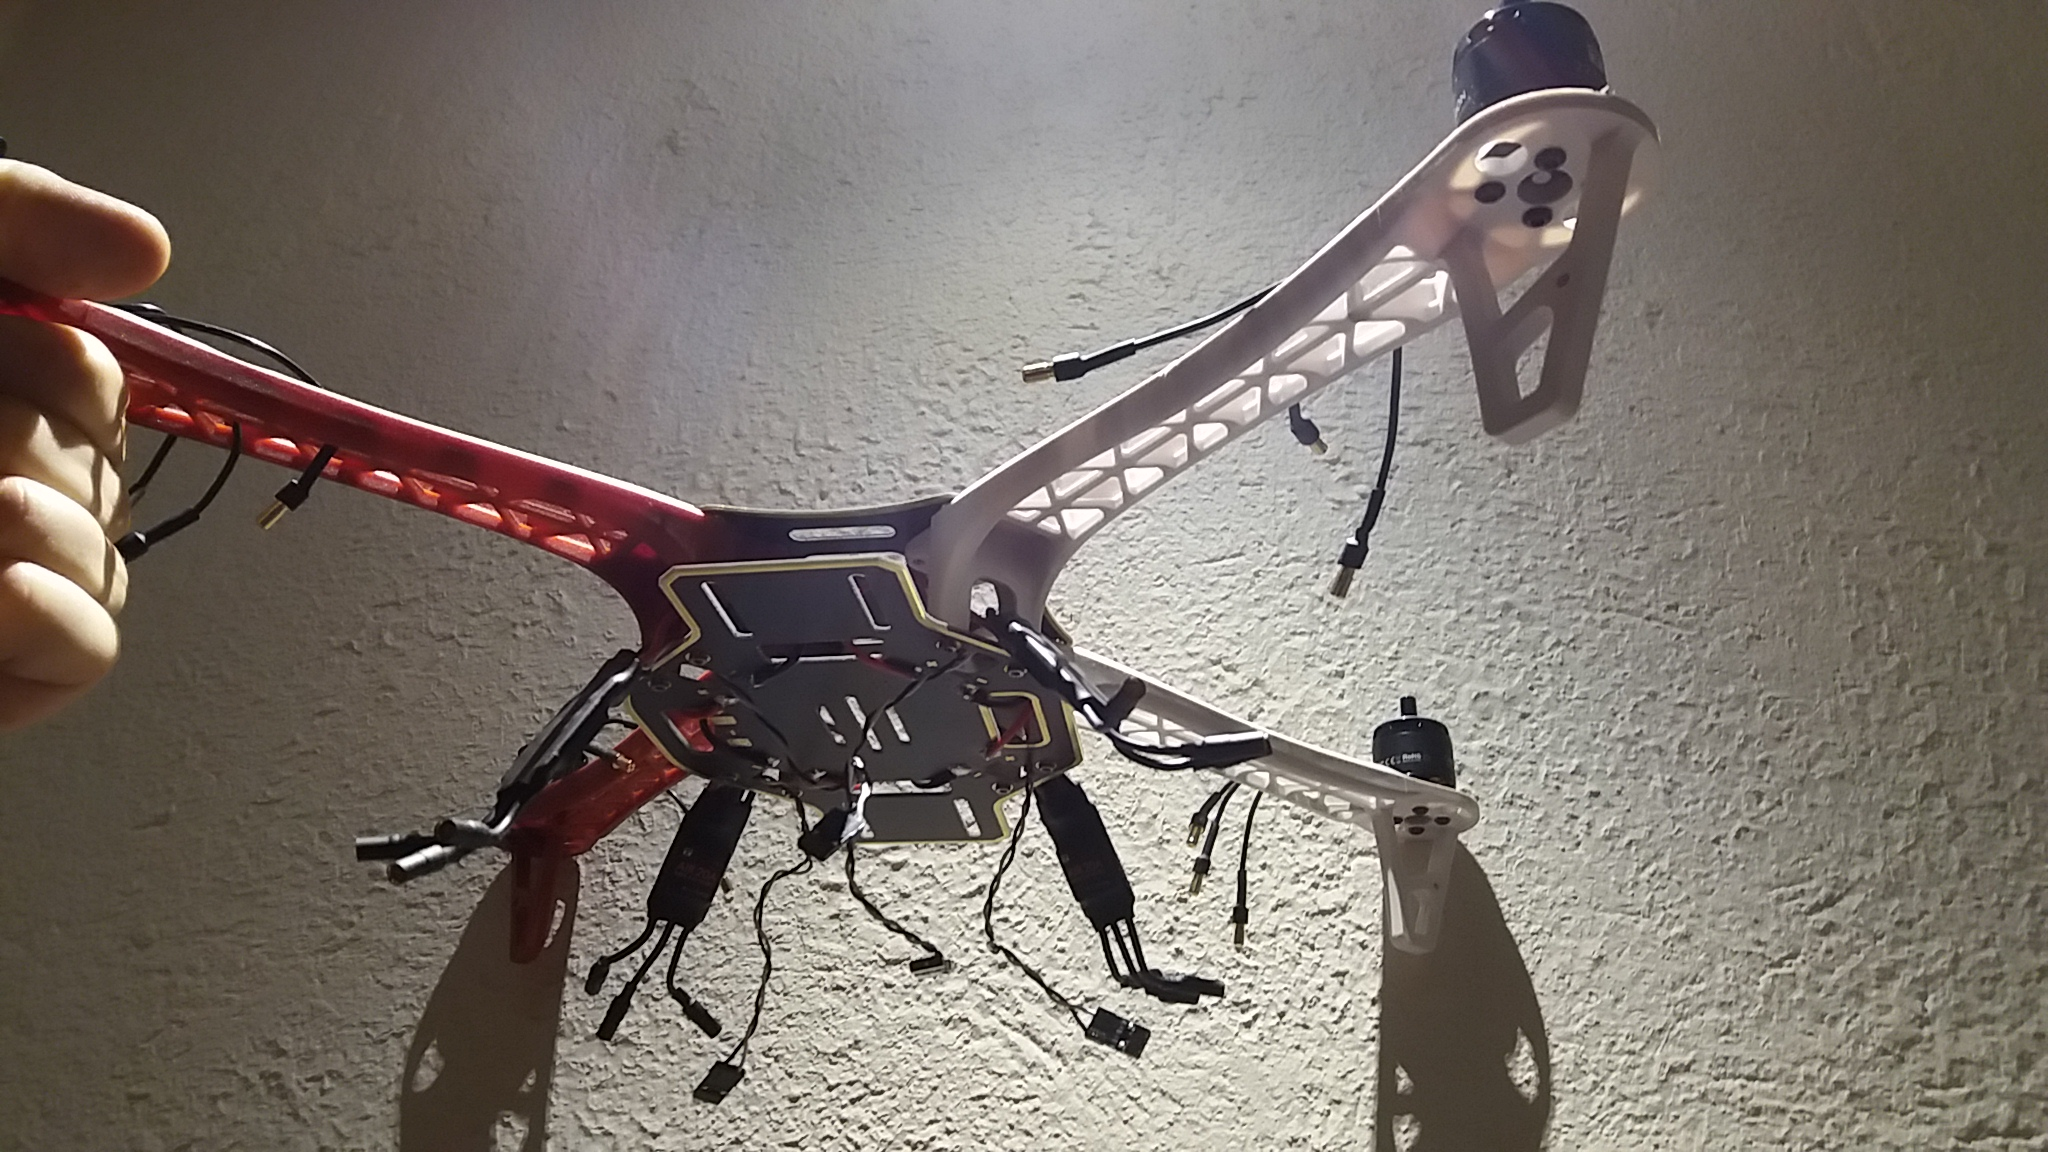
\includegraphics[scale=0.1]{images/drone-build-esc-3phaseunconnected.jpg}
\caption{Adding the ESCs. Motors require 3-phase power}
\label{fig:ESCs_uplugged}
\end{subfigure}
\begin{subfigure}{0.5\textwidth}
\centering
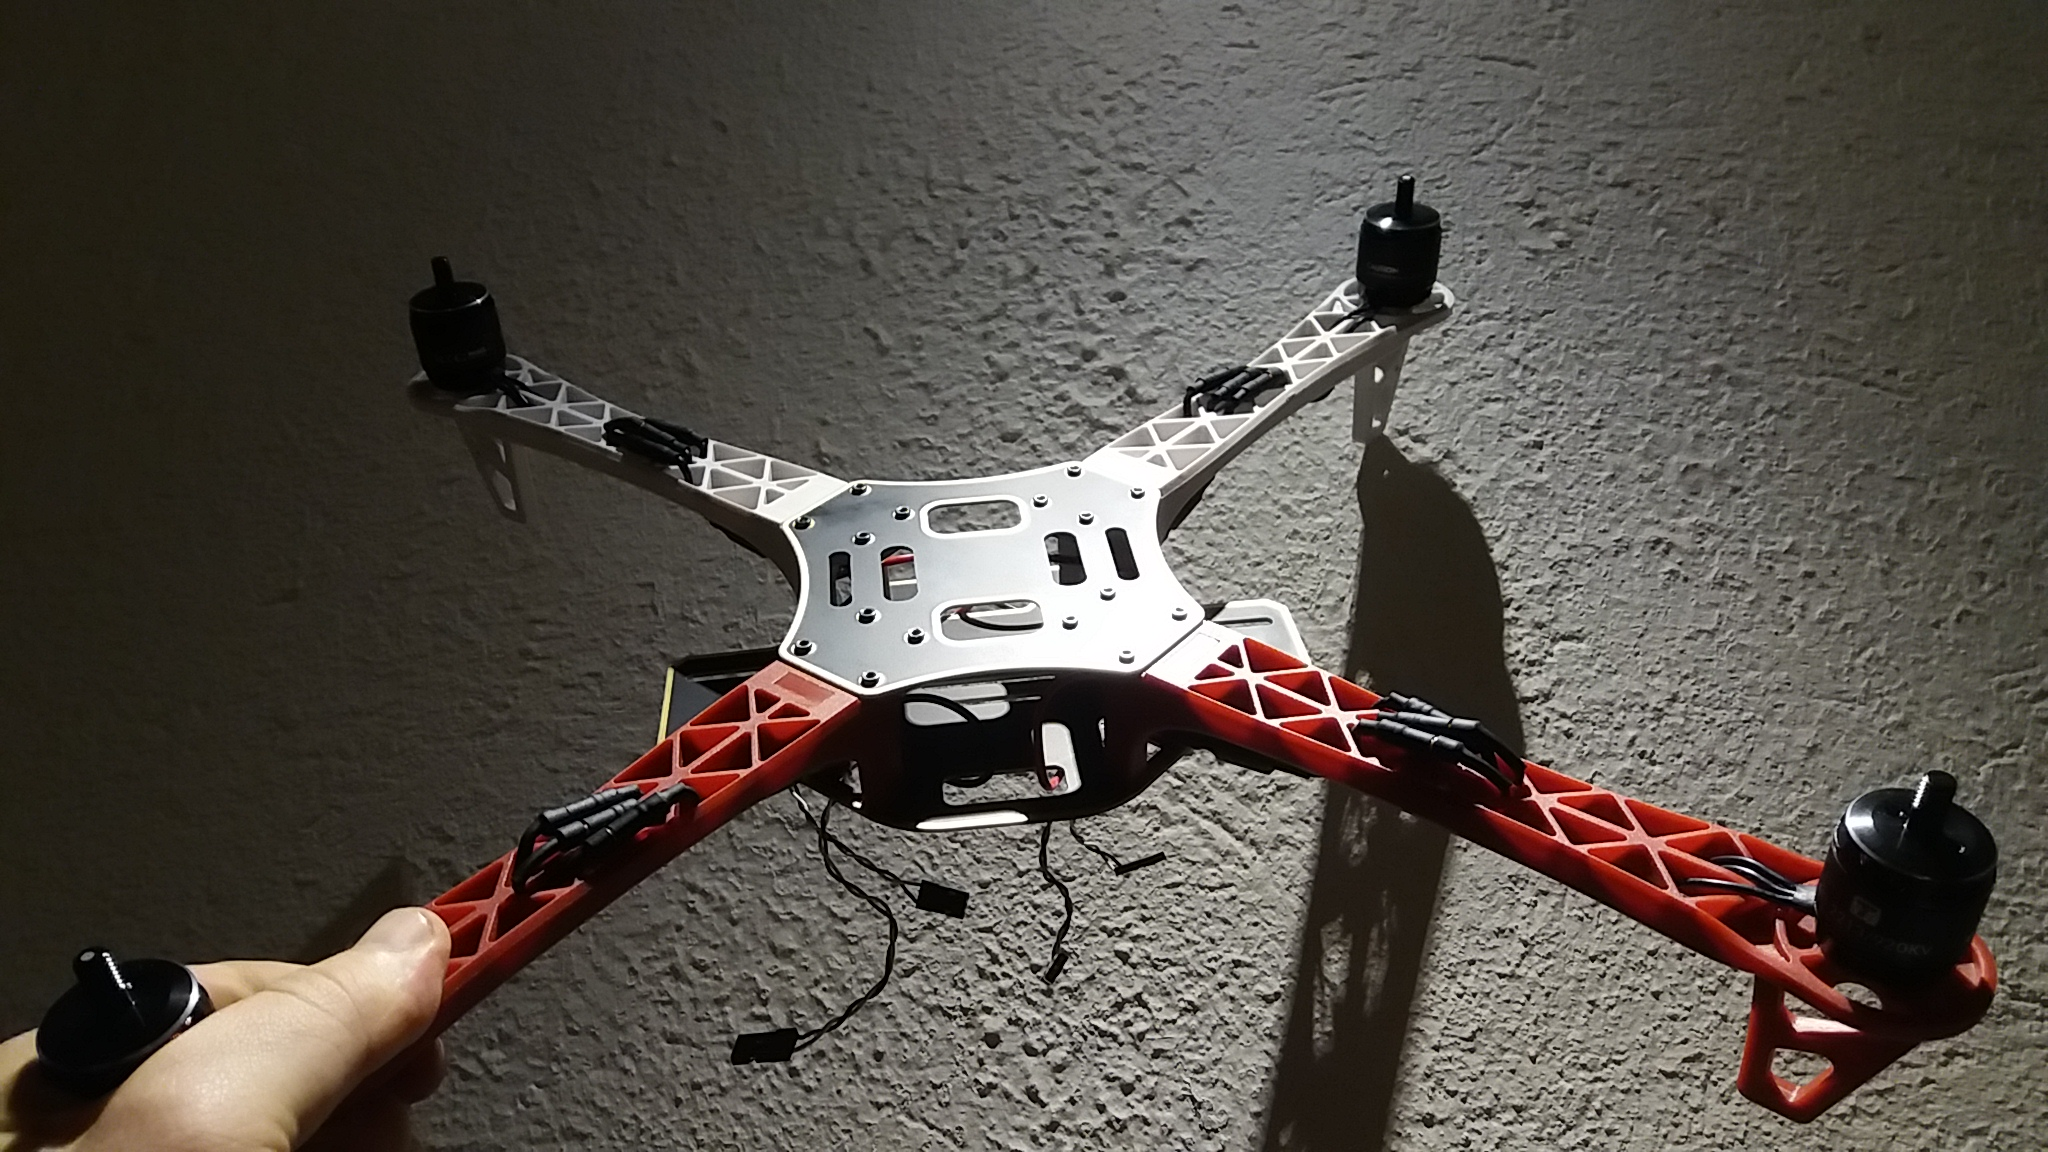
\includegraphics[scale=0.1]{images/drone-build-esc-3phaseconnected.jpg}
\caption{Power leads plugged in and secured}
\label{fig:ESCs_plugged}
\end{subfigure}
\caption{ESCs}
\label{fig:ESC}
\end{figure}

The leads are easy to plug/unplug. Any two phase leads can be swapped to change motor direction as in Figure \ref{fig:ESC}.\\

\begin{figure}[H]
\begin{subfigure}{0.5\textwidth}
\centering
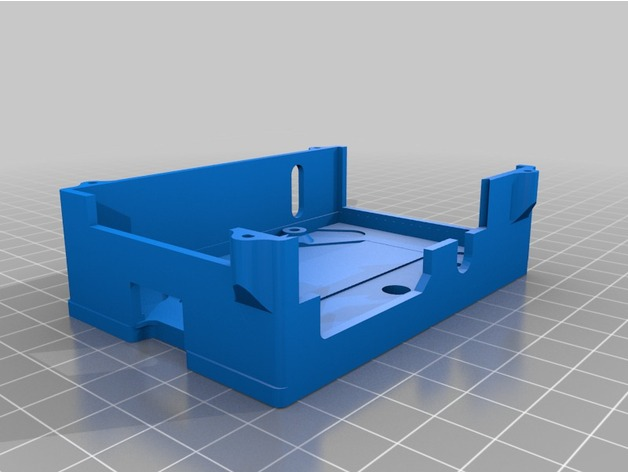
\includegraphics[scale=0.25]{images/drone-build-3d-case-render.jpg}
\caption{Case render}
\label{fig:fcarpc1}
\end{subfigure}
\begin{subfigure}{0.5\textwidth}
\centering
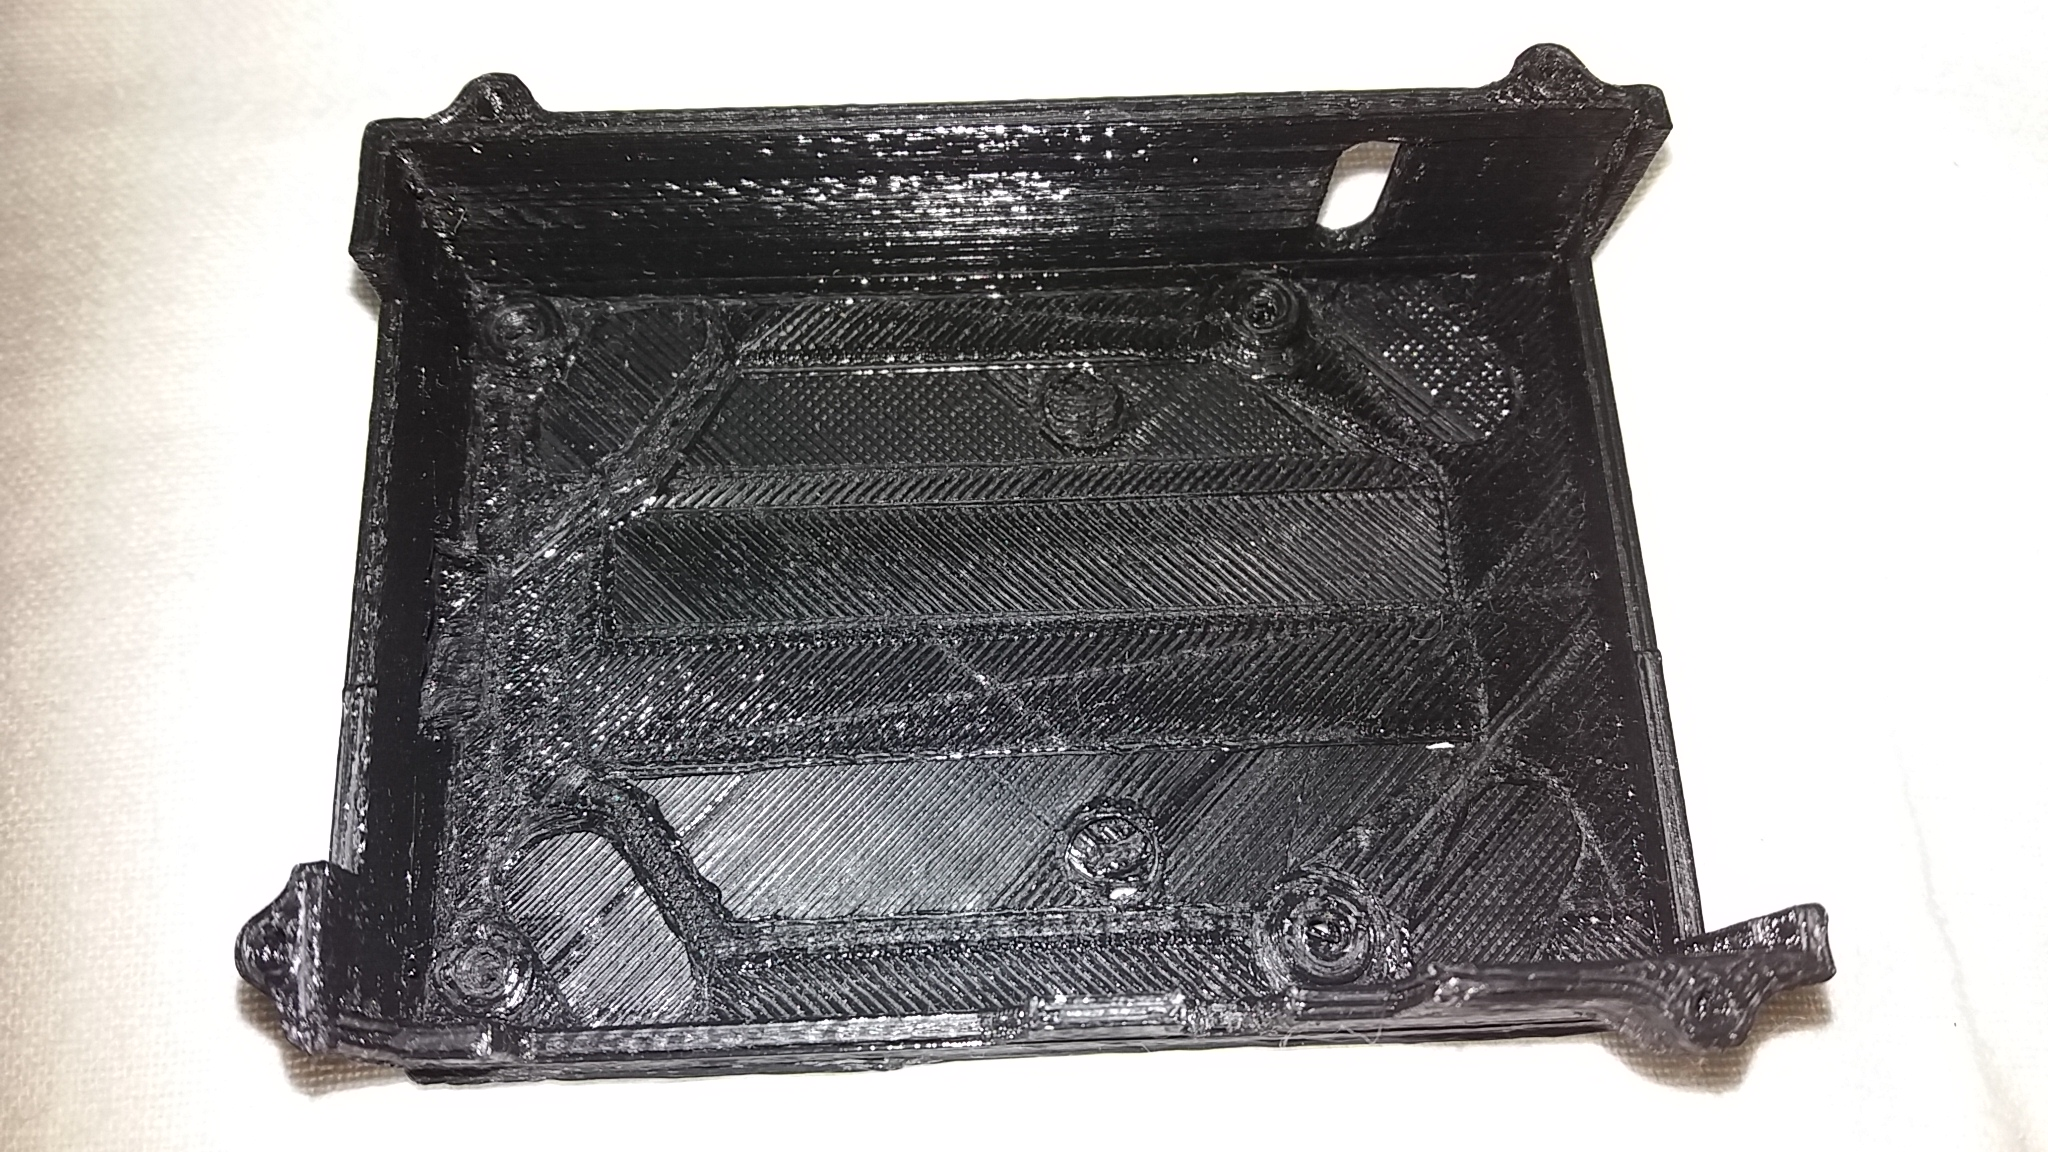
\includegraphics[scale=0.1]{images/drone-build-3dcase.jpg}
\caption{3D printed case for Raspberry Pi and Navio2.}
\label{fig:fcarpc2}
\end{subfigure}
\caption{Flight controller and Raspberry Pi case}
\label{fig:fcarpc}
\end{figure}

A housing is needed to protect the exposed electronics from the elements as shown in Figure \ref{fig:fcarpc}. Also, dramatic airflow can affect the barometer readings. Thus, a 3D printed case was made.

\begin{figure}[H]
\begin{subfigure}{0.5\textwidth}
\centering
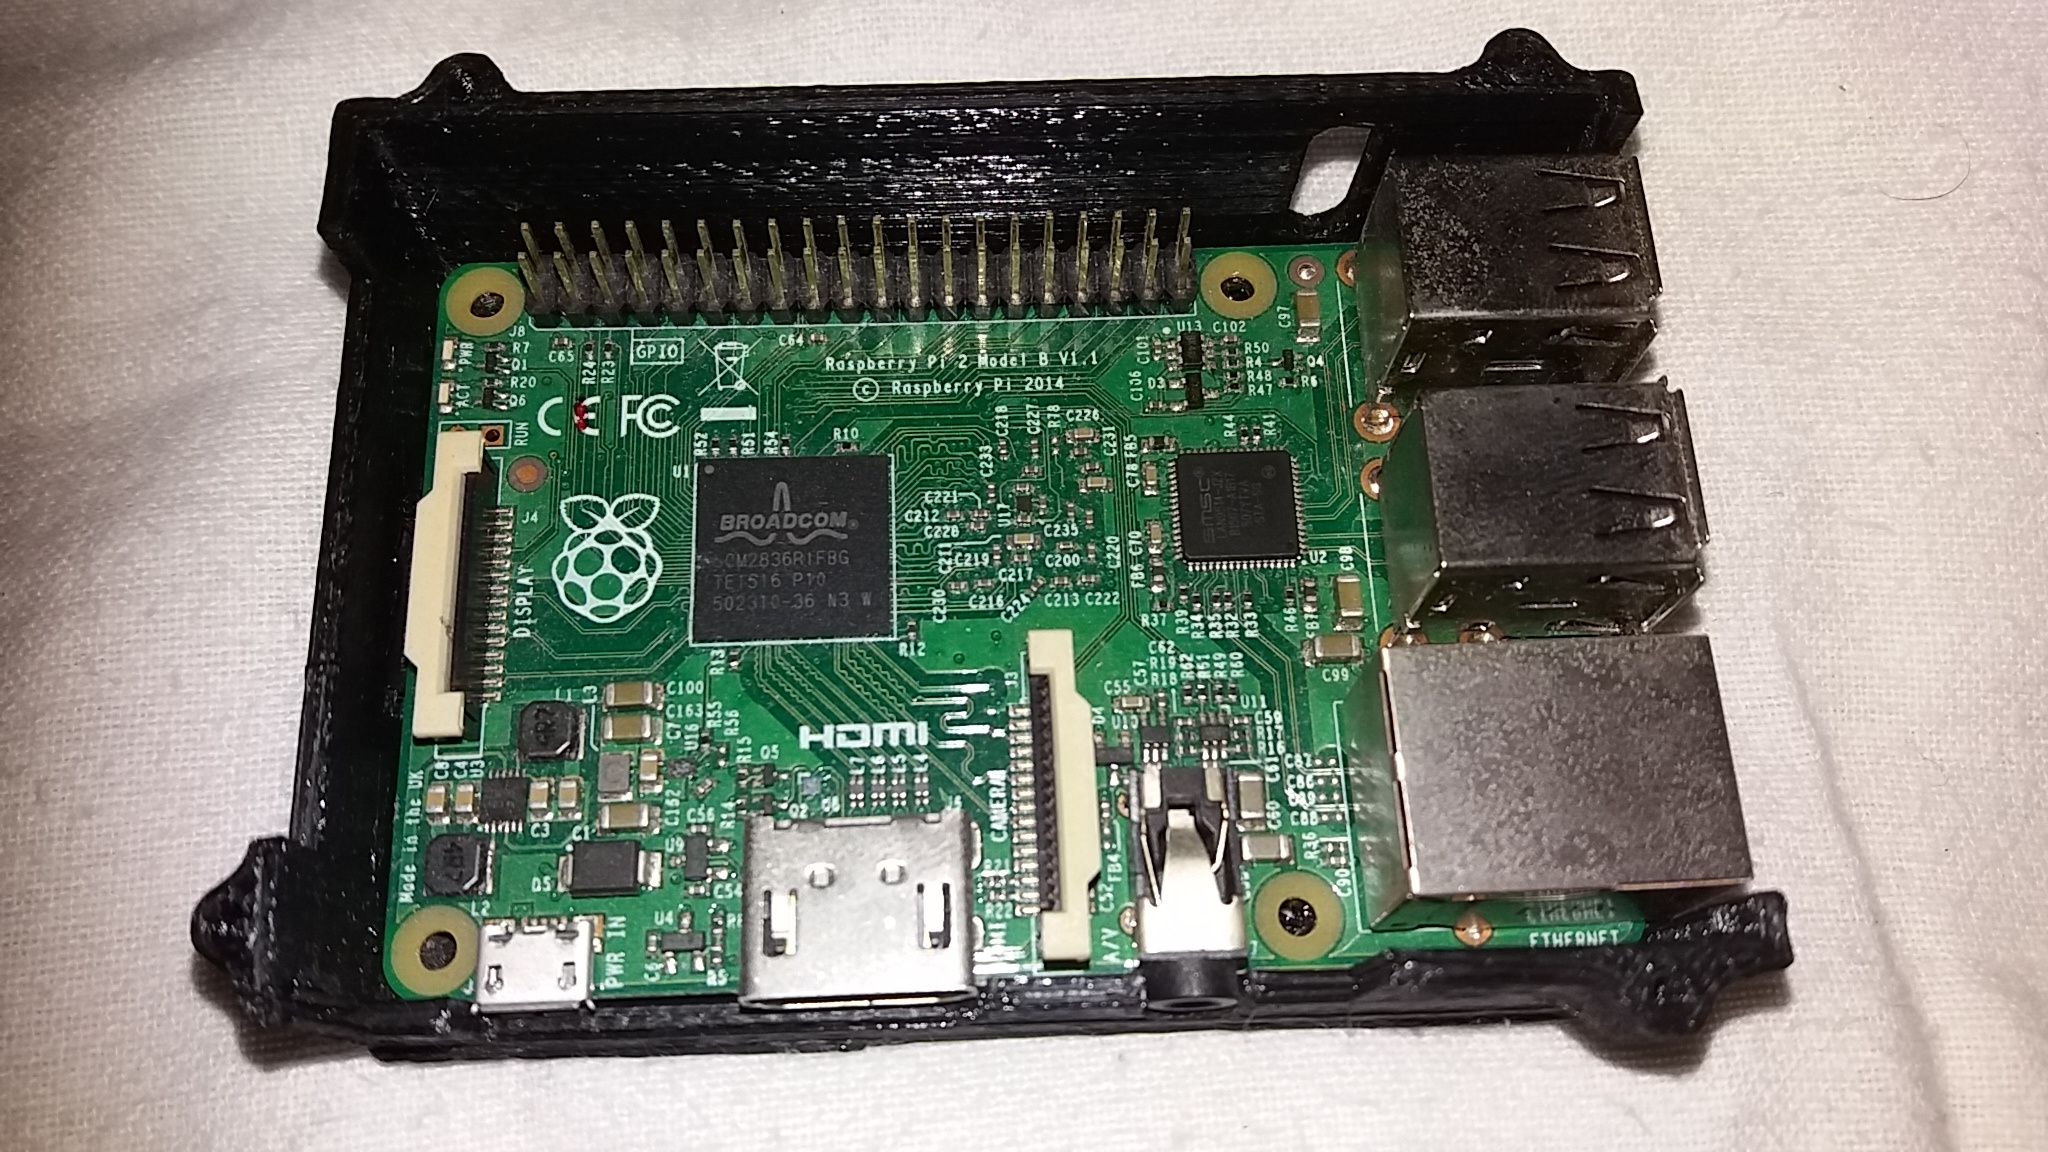
\includegraphics[scale=0.1]{images/drone-build-3dcase-pi.jpg}
\caption{Putting the Pi in the case.}
\label{fig:insertion_pi}
\end{subfigure}
\begin{subfigure}{0.5\textwidth}
\centering
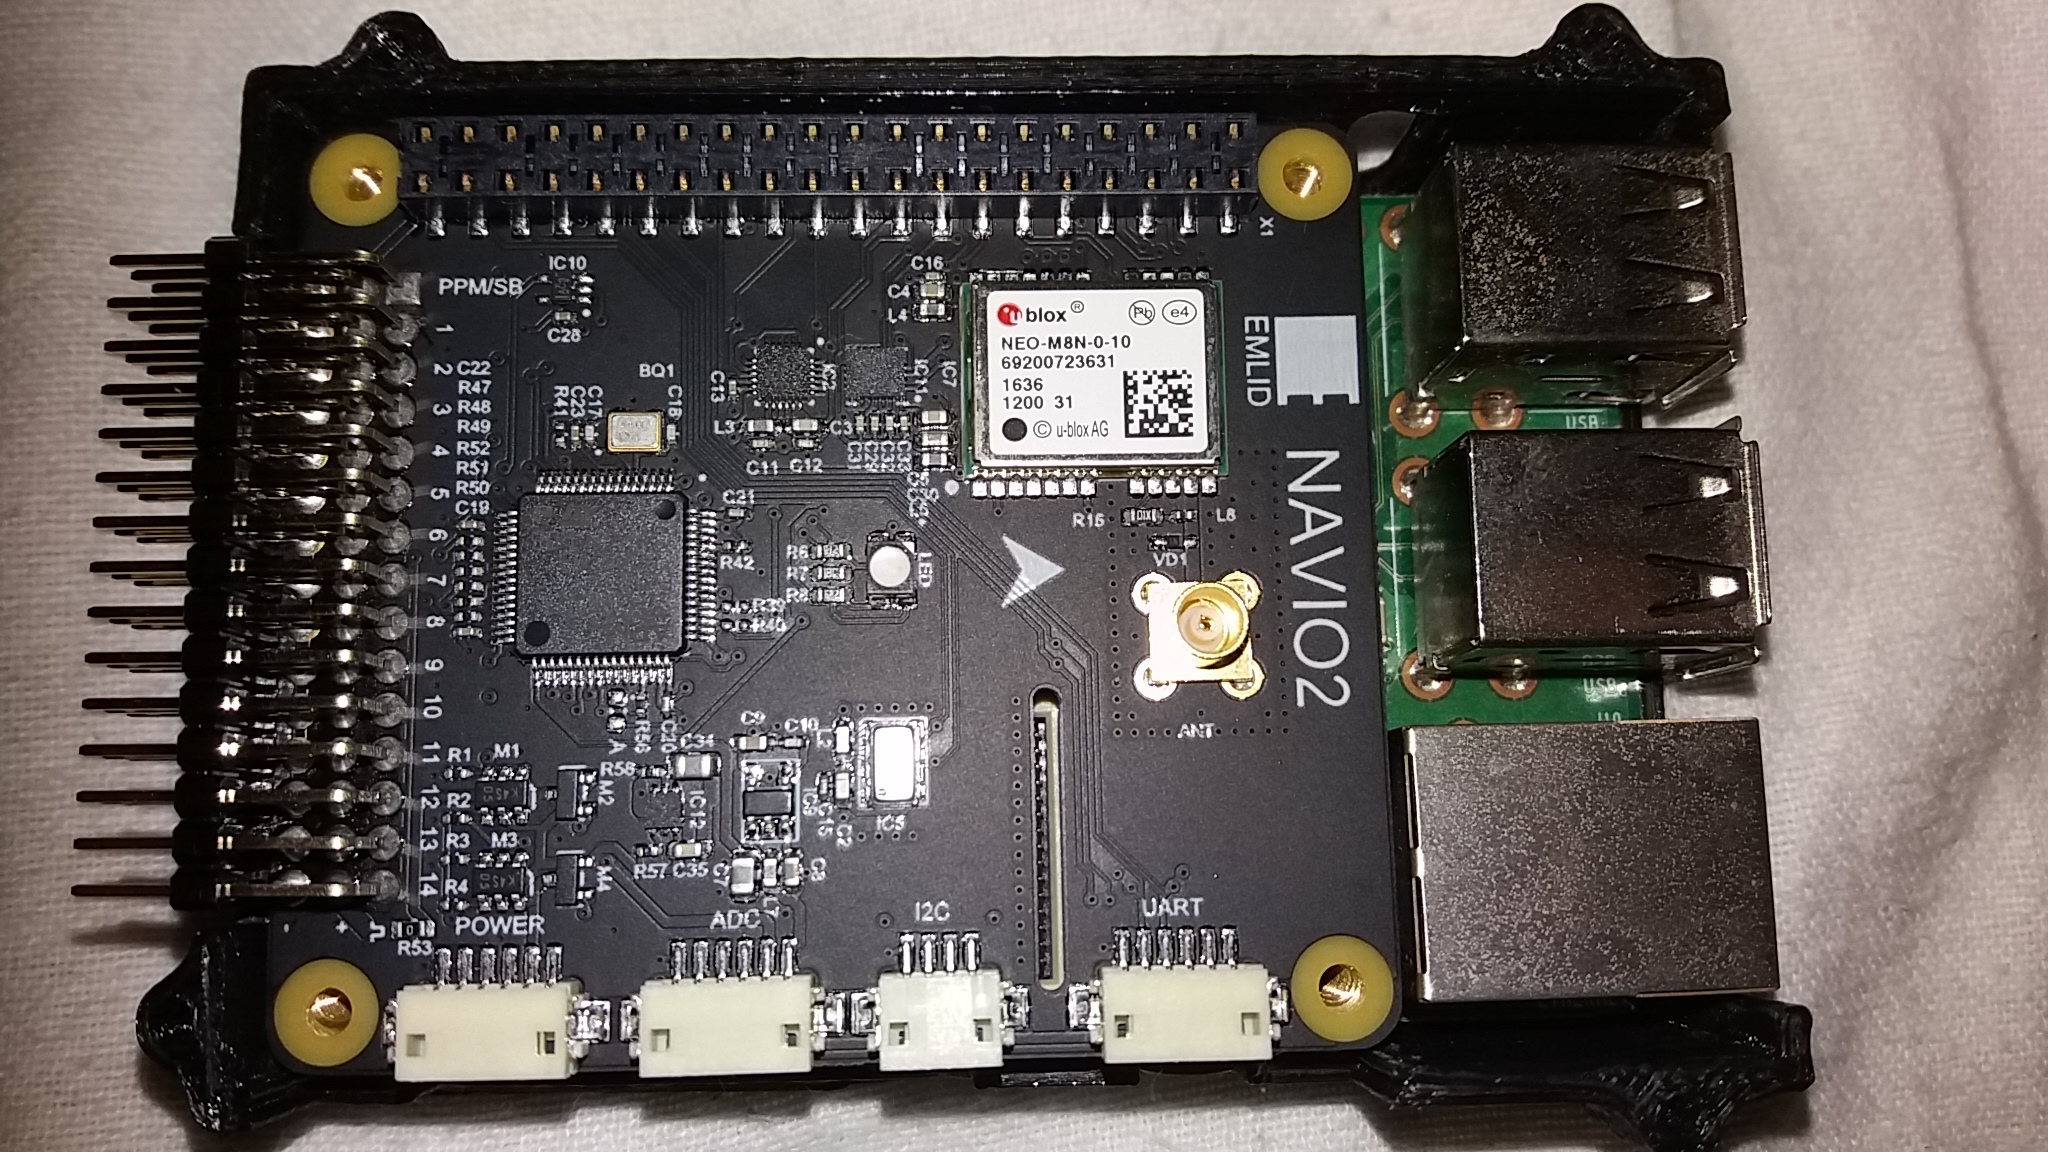
\includegraphics[scale=0.1]{images/drone-build-3dcase-pi-navio.jpg}
\caption{Fitting the Navio2 flight controller on top.}
\label{fig:insertion_navio}
\end{subfigure}
\caption{Inserting the sensitive electronics.}
\label{fig:insertion}
\end{figure}

The Navio2 flight controller fits perfectly onto the Raspberry Pi's 40-pin header in Figure \ref{fig:insertion_navio}. It also uses every signal pin, except for one. The Navio2 communicates directly with the Broadcom CPU on the Pi, resulting in a multi-processor system. The greatest significance in this case is that flight variables can be monitored and controlled. It is non-trivial in standalone flight controllers, as the on-board firmware has to be modified with utmost care.

\begin{figure}[H]
\begin{subfigure}{0.5\textwidth}
\centering
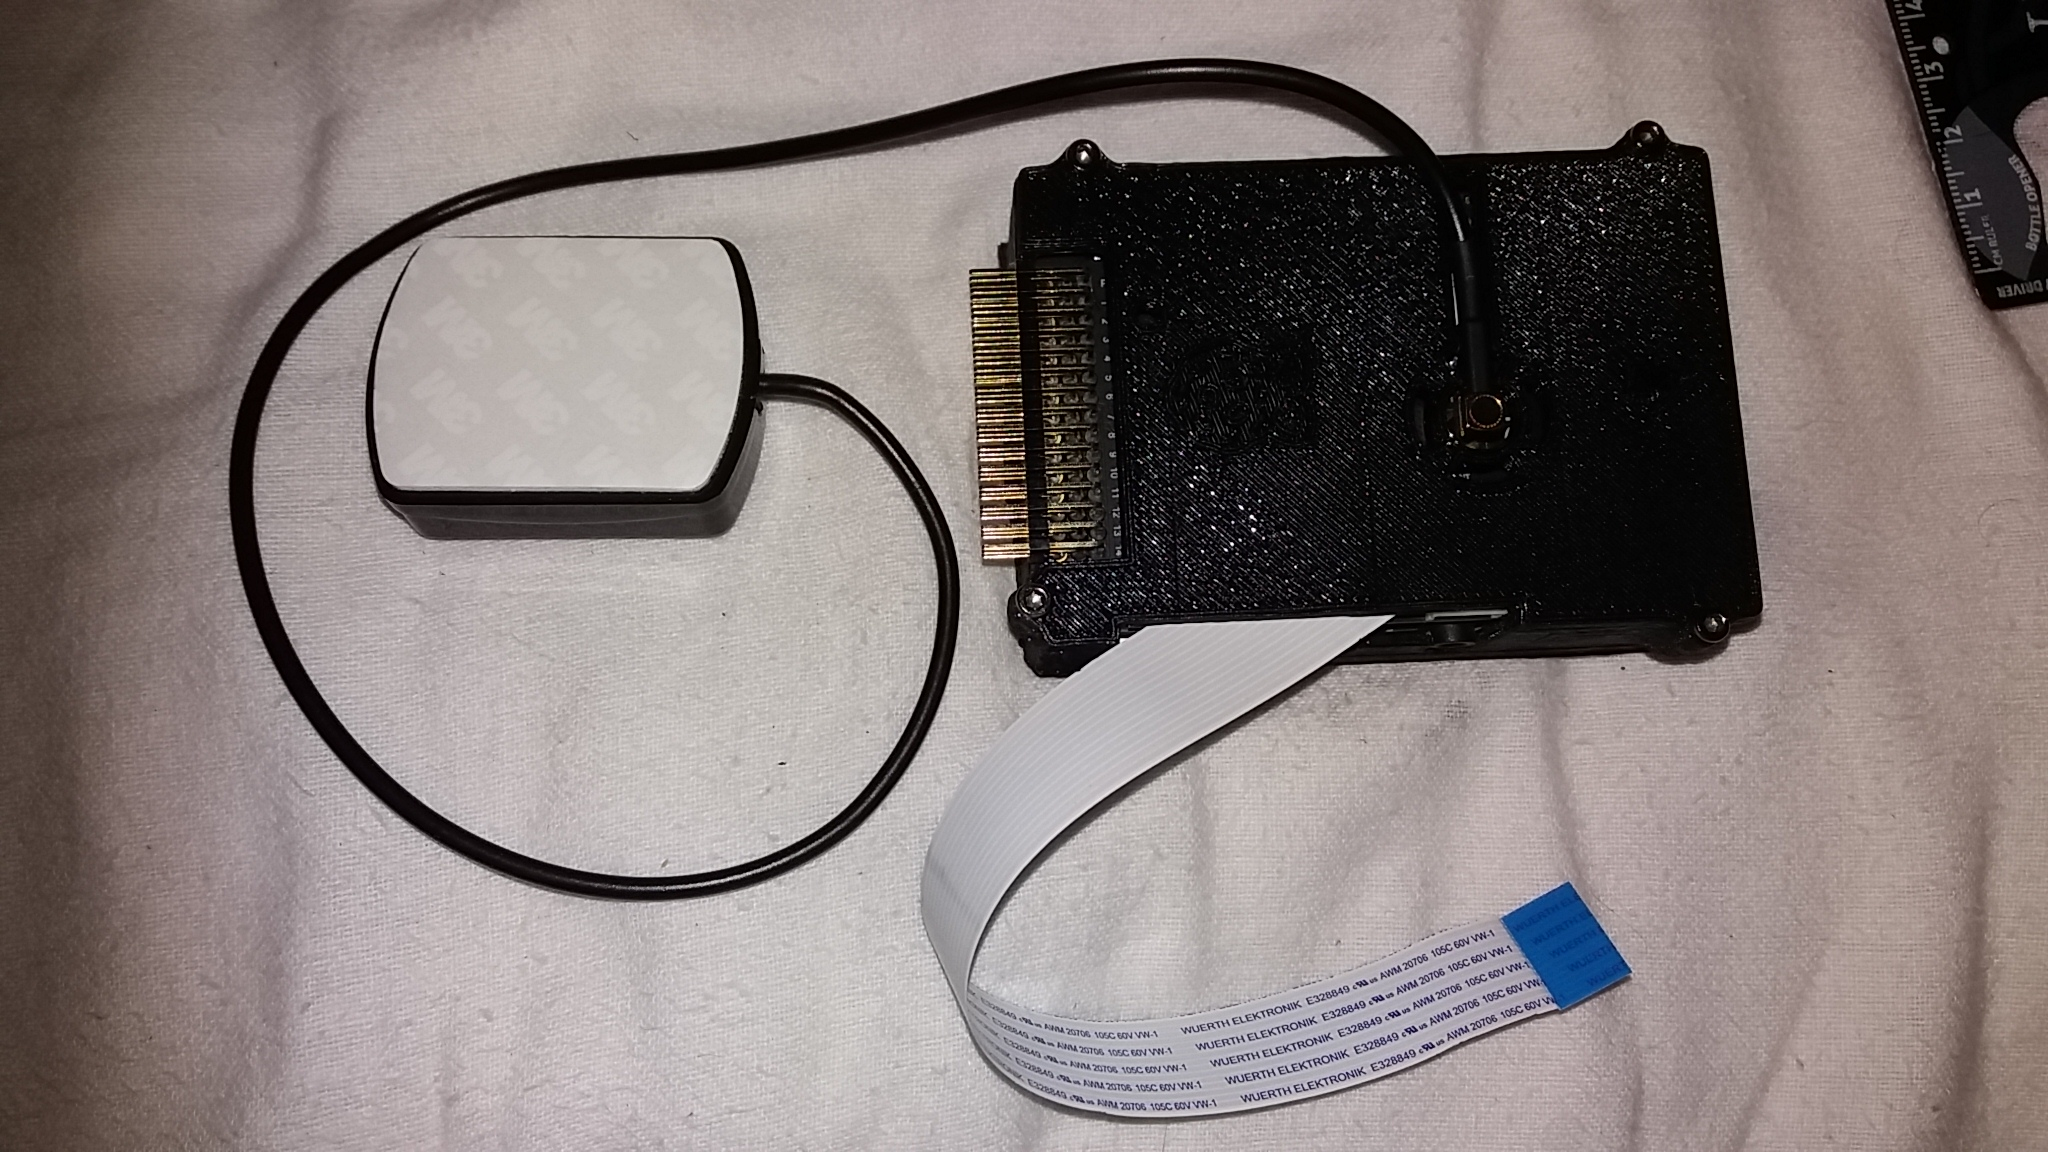
\includegraphics[scale=0.1]{images/drone-build-3dcase-gps.jpg}
\caption{Connecting Ublox Neo-7 GPS antenna and 15-pin camera CSI ribbon cable.}
\label{fig:stab_gps}
\end{subfigure}
\begin{subfigure}{0.5\textwidth}
\centering
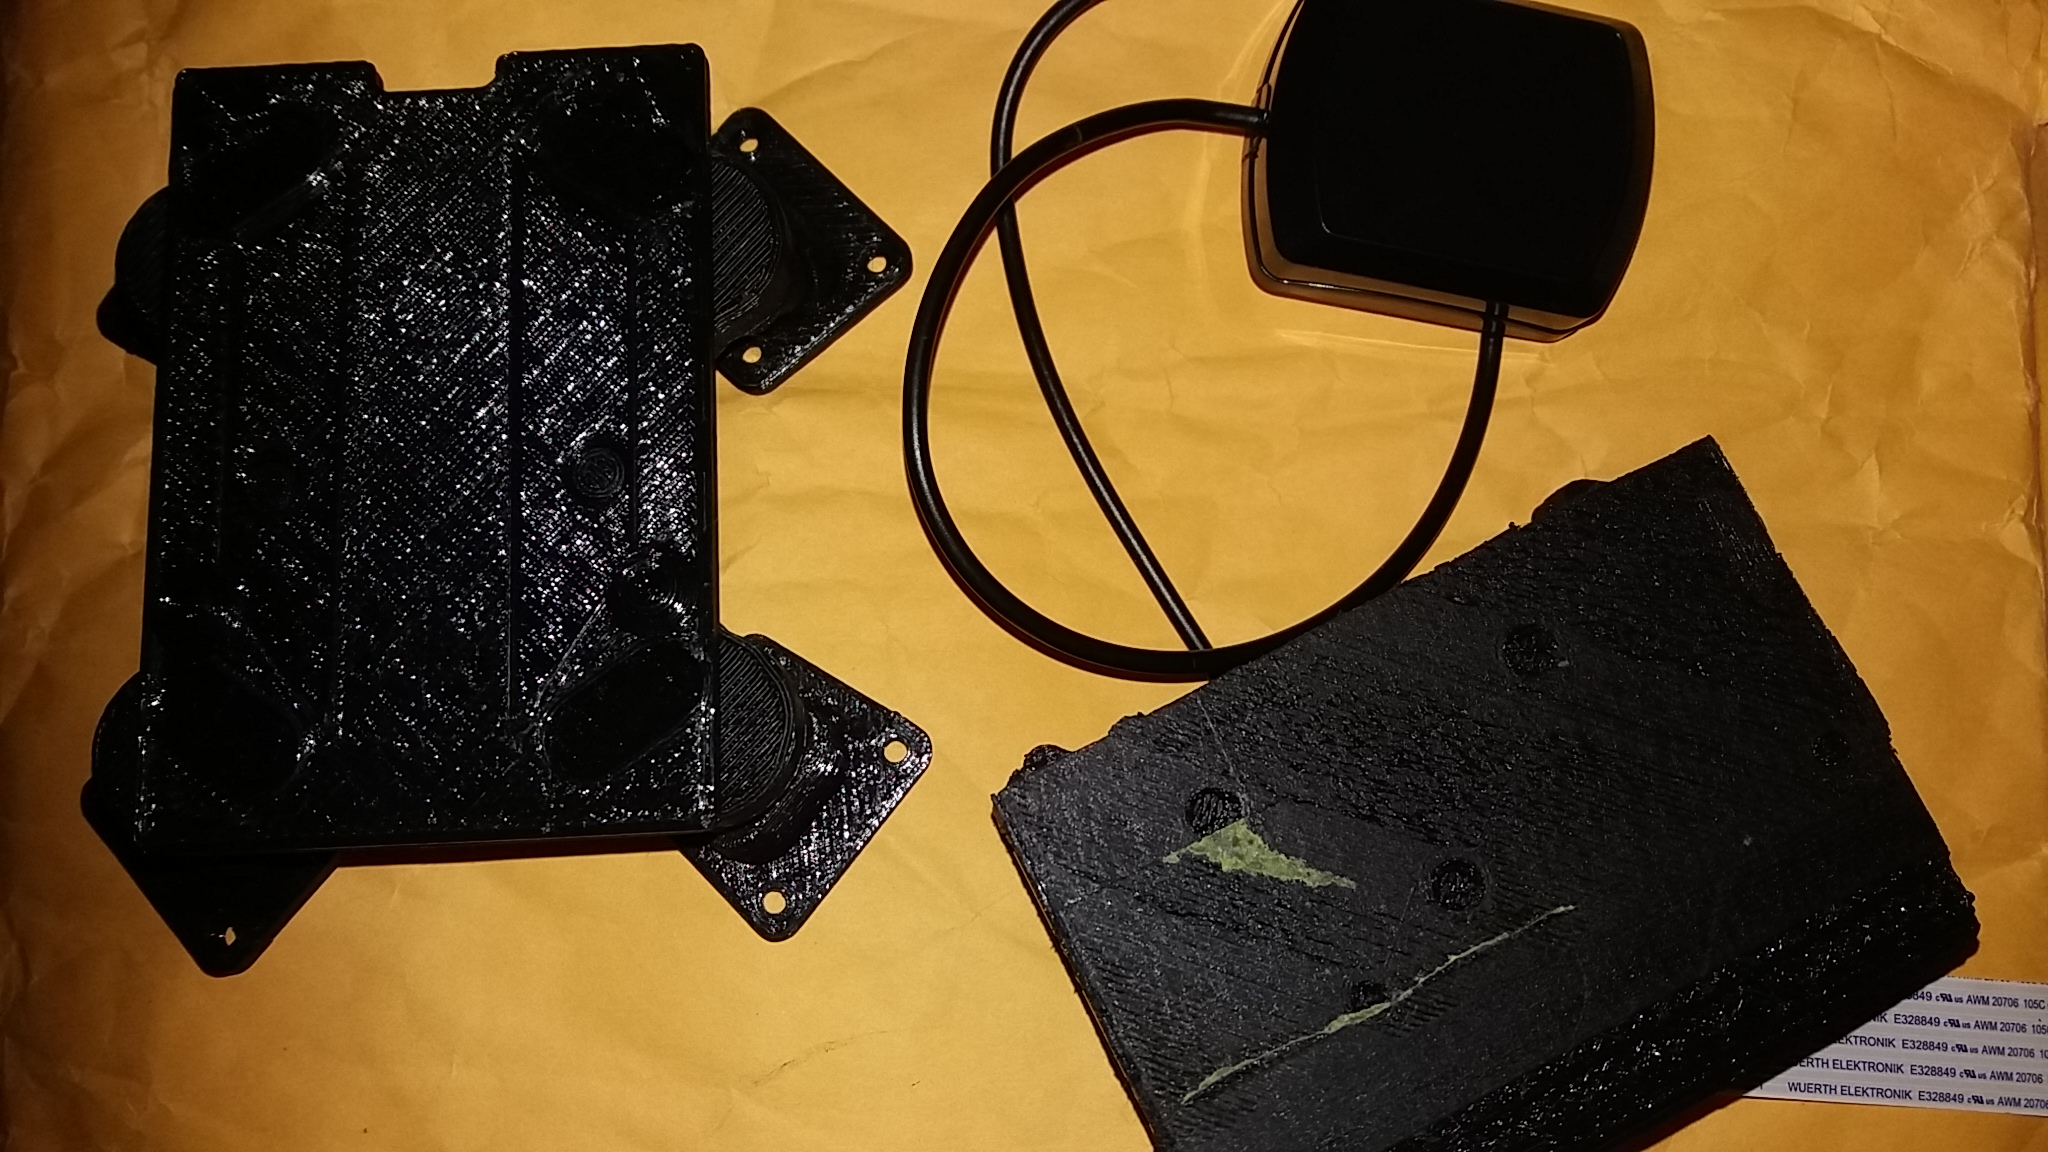
\includegraphics[scale=0.1]{images/drone-build-3dplatform.jpg}
\caption{Case and platform}
\label{fig:stab_case_plat}
\end{subfigure}
\caption{Putting the case and platform together}
\label{fig:stabilize_platform}
\end{figure}

The GPS antenna lead fits snugly onto an SMA connector in Figure \ref{fig:stab_gps}, and is exposed in such a way as to leave enough freedom for the cable to bend, but not wear as if it were rigidly attached.

\begin{figure}[H]
\begin{subfigure}{0.5\textwidth}
\centering
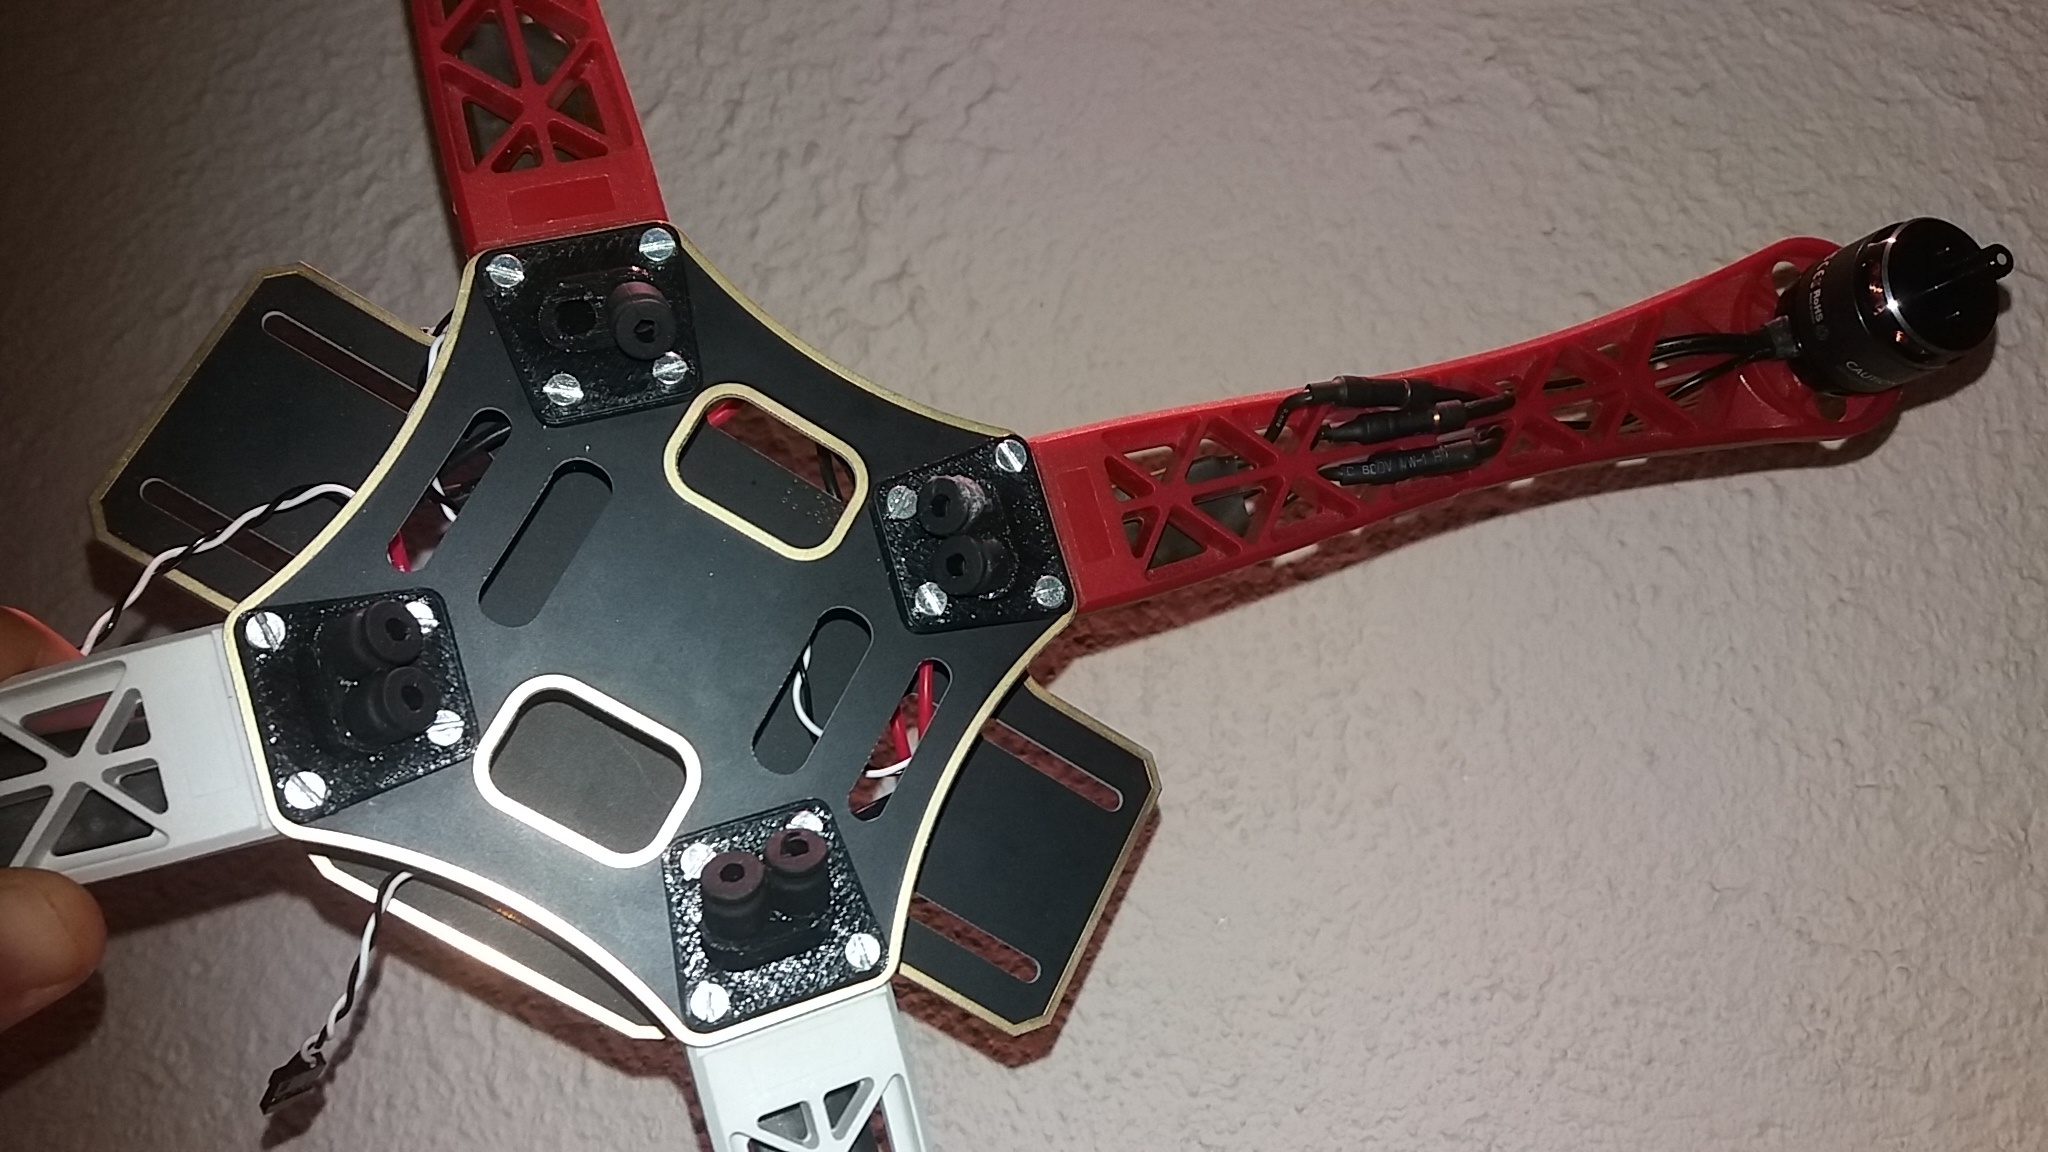
\includegraphics[scale=0.1]{images/drone-build-feet.jpg}
\caption{Added feet for platform.} 
\label{fig:feet}
\end{subfigure}
\begin{subfigure}{0.5\textwidth}
\centering
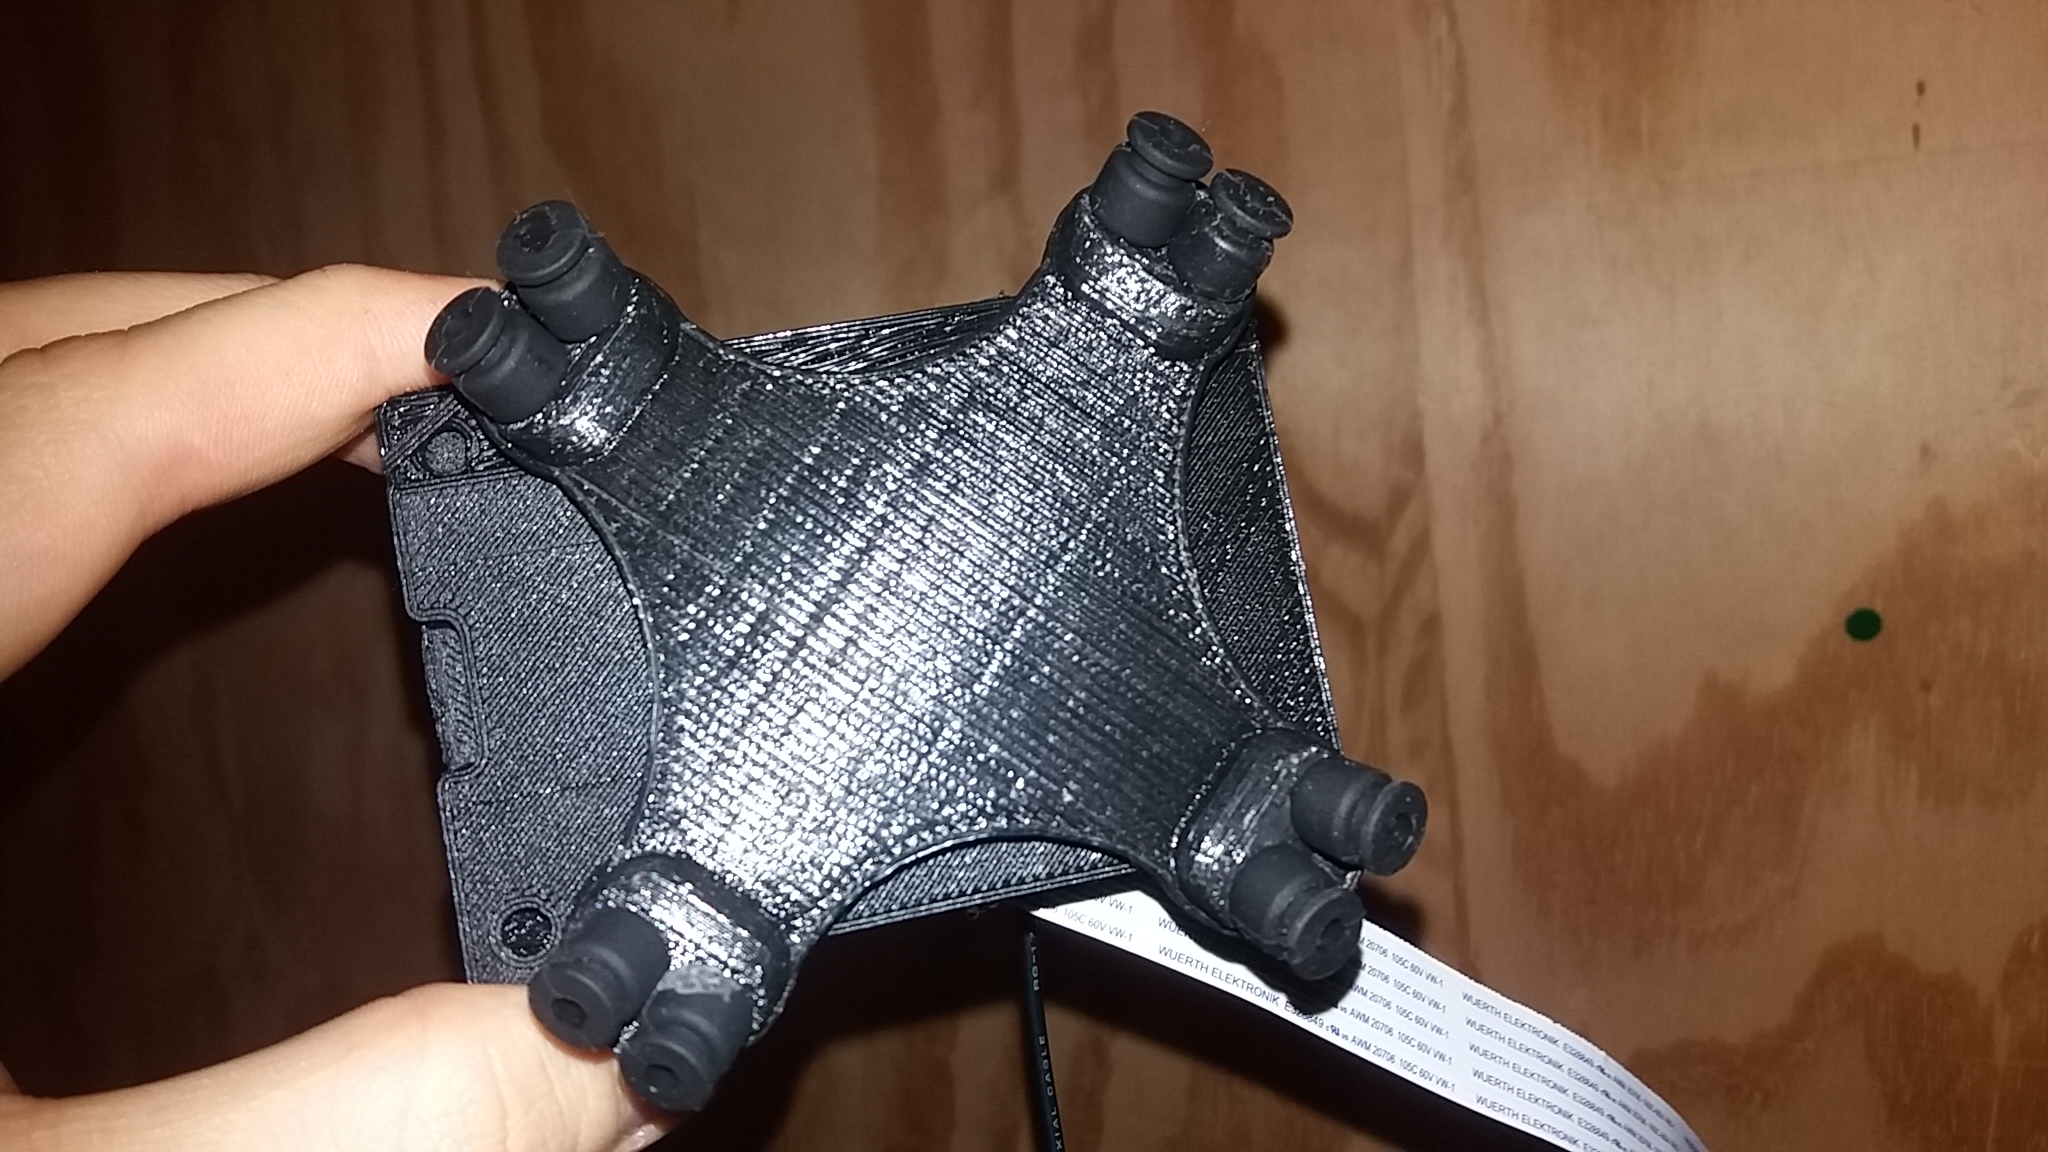
\includegraphics[scale=0.1]{images/drone-build-damper-balls.jpg}
\caption{Rubber vibration damper balls for platform.}
\label{fig:balls}
\end{subfigure}
\caption{Isolating vibrations between flight controller and the rest of the drone}
\label{fig:stabilize_platform}
\end{figure}

One of the biggest problems in a drone is the vibrations emanating from the motors, travelling along the frame and affecting the flight controller. If not isolated from the flight controller, they induce a disturbance to the PID loop since the accuracy of the gyroscope, accelerometer and barometer readings are affected. In some cases, disturbed more than the PID loop can reasonably determine the current state of the drone.\\

Thus, damper balls can be used to isolate vibrations significantly from the flight controller.

\begin{figure}[H]
\begin{subfigure}{0.5\textwidth}
\centering
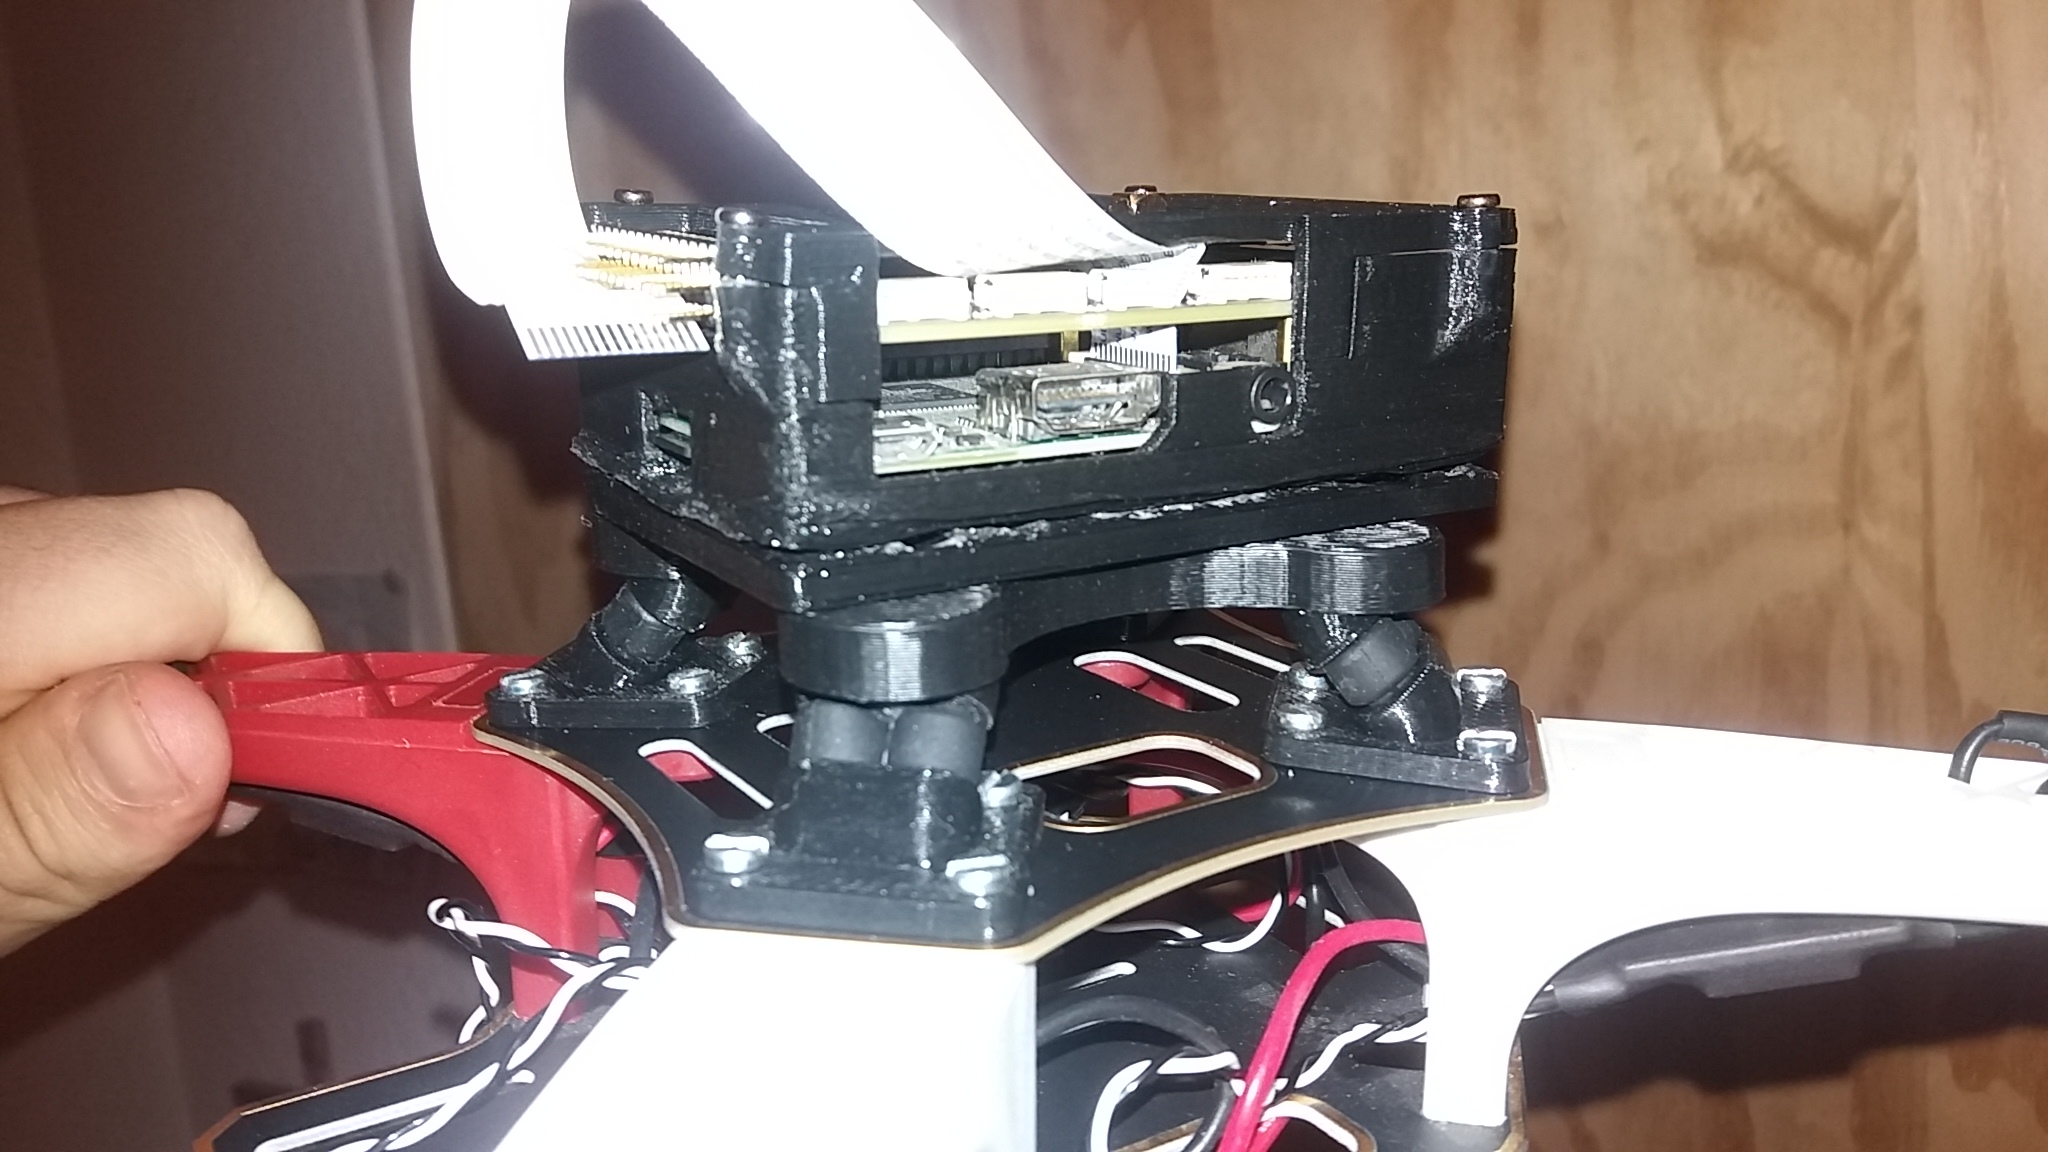
\includegraphics[scale=0.1]{images/drone-build-case-ondrone.jpg}
\caption{Attaching 3D printed case and platform to drone.}
\label{fig:attach_case_drone}
\end{subfigure}
\begin{subfigure}{0.5\textwidth}
\centering
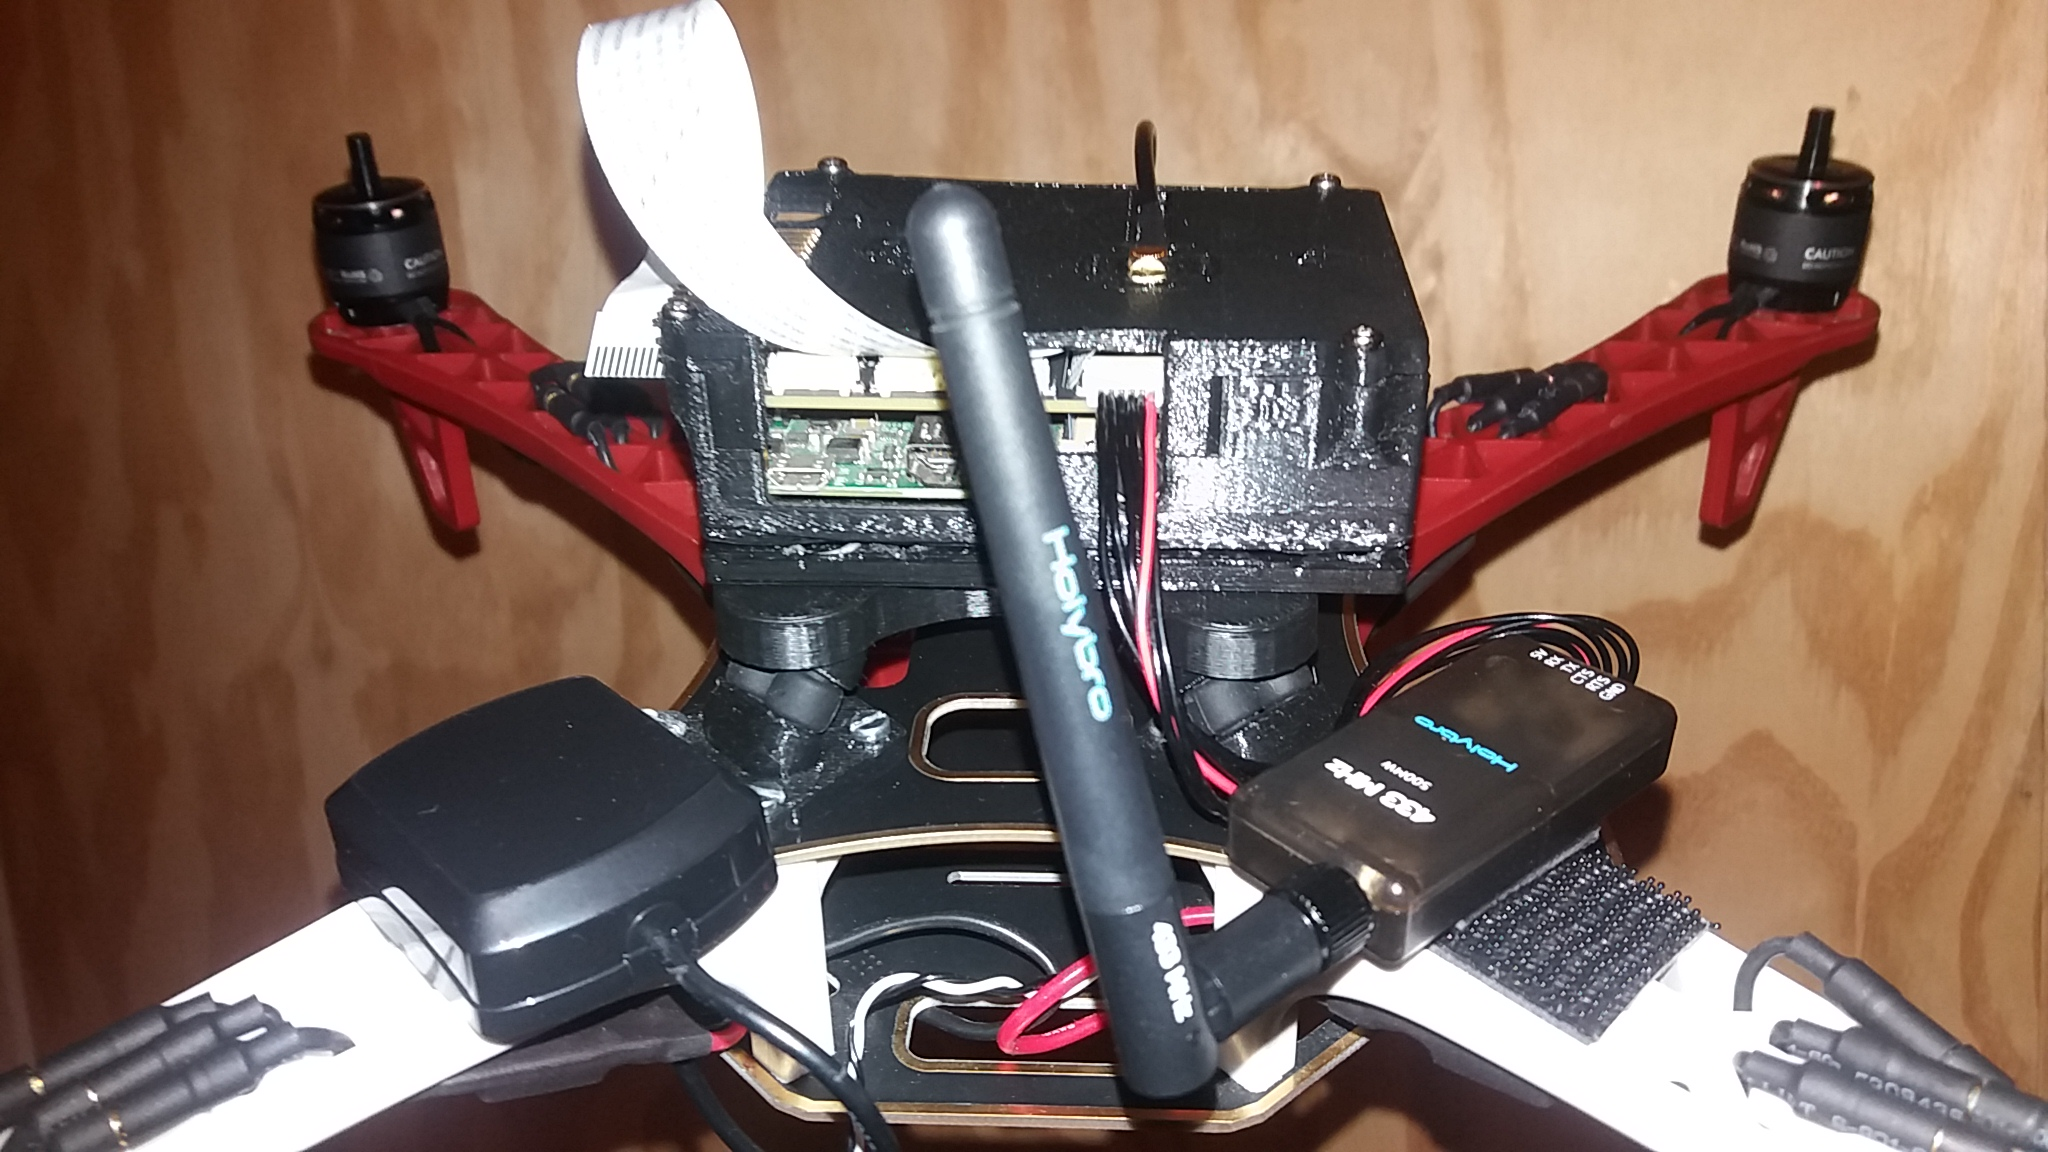
\includegraphics[scale=0.1]{images/drone-build-433.jpg}
\caption{Adding 433MHz telemtery to drone.}
\label{fig:attach_433}
\end{subfigure}
\caption{Isolating vibrations between flight controller and the rest of the drone}
\label{fig:attach_case_433}
\end{figure}

Finally, the 3D printed enclosure is attached to the drone in Figure \ref{fig:attach_case_drone}. Also, the drone can communicate via wifi as its medium of wireless telemetry; but the interference from other devices in the crowded 2.4 GHz ISM band drastically reduces range -- especially from the handheld remote controller. That, and the dongles I had available seemed to work only for about 10 m.\\

Thus, I connected a 433 MHz 100mW transceiver that communicates at 56400 baud to the GCS as in Figure \ref{fig:attach_433}. Real-time telemtery to a ground station is useful for pre-flight checks, in-flight monitoring and control, and missions.

\begin{figure}[H]
\begin{subfigure}{0.5\textwidth}
\centering
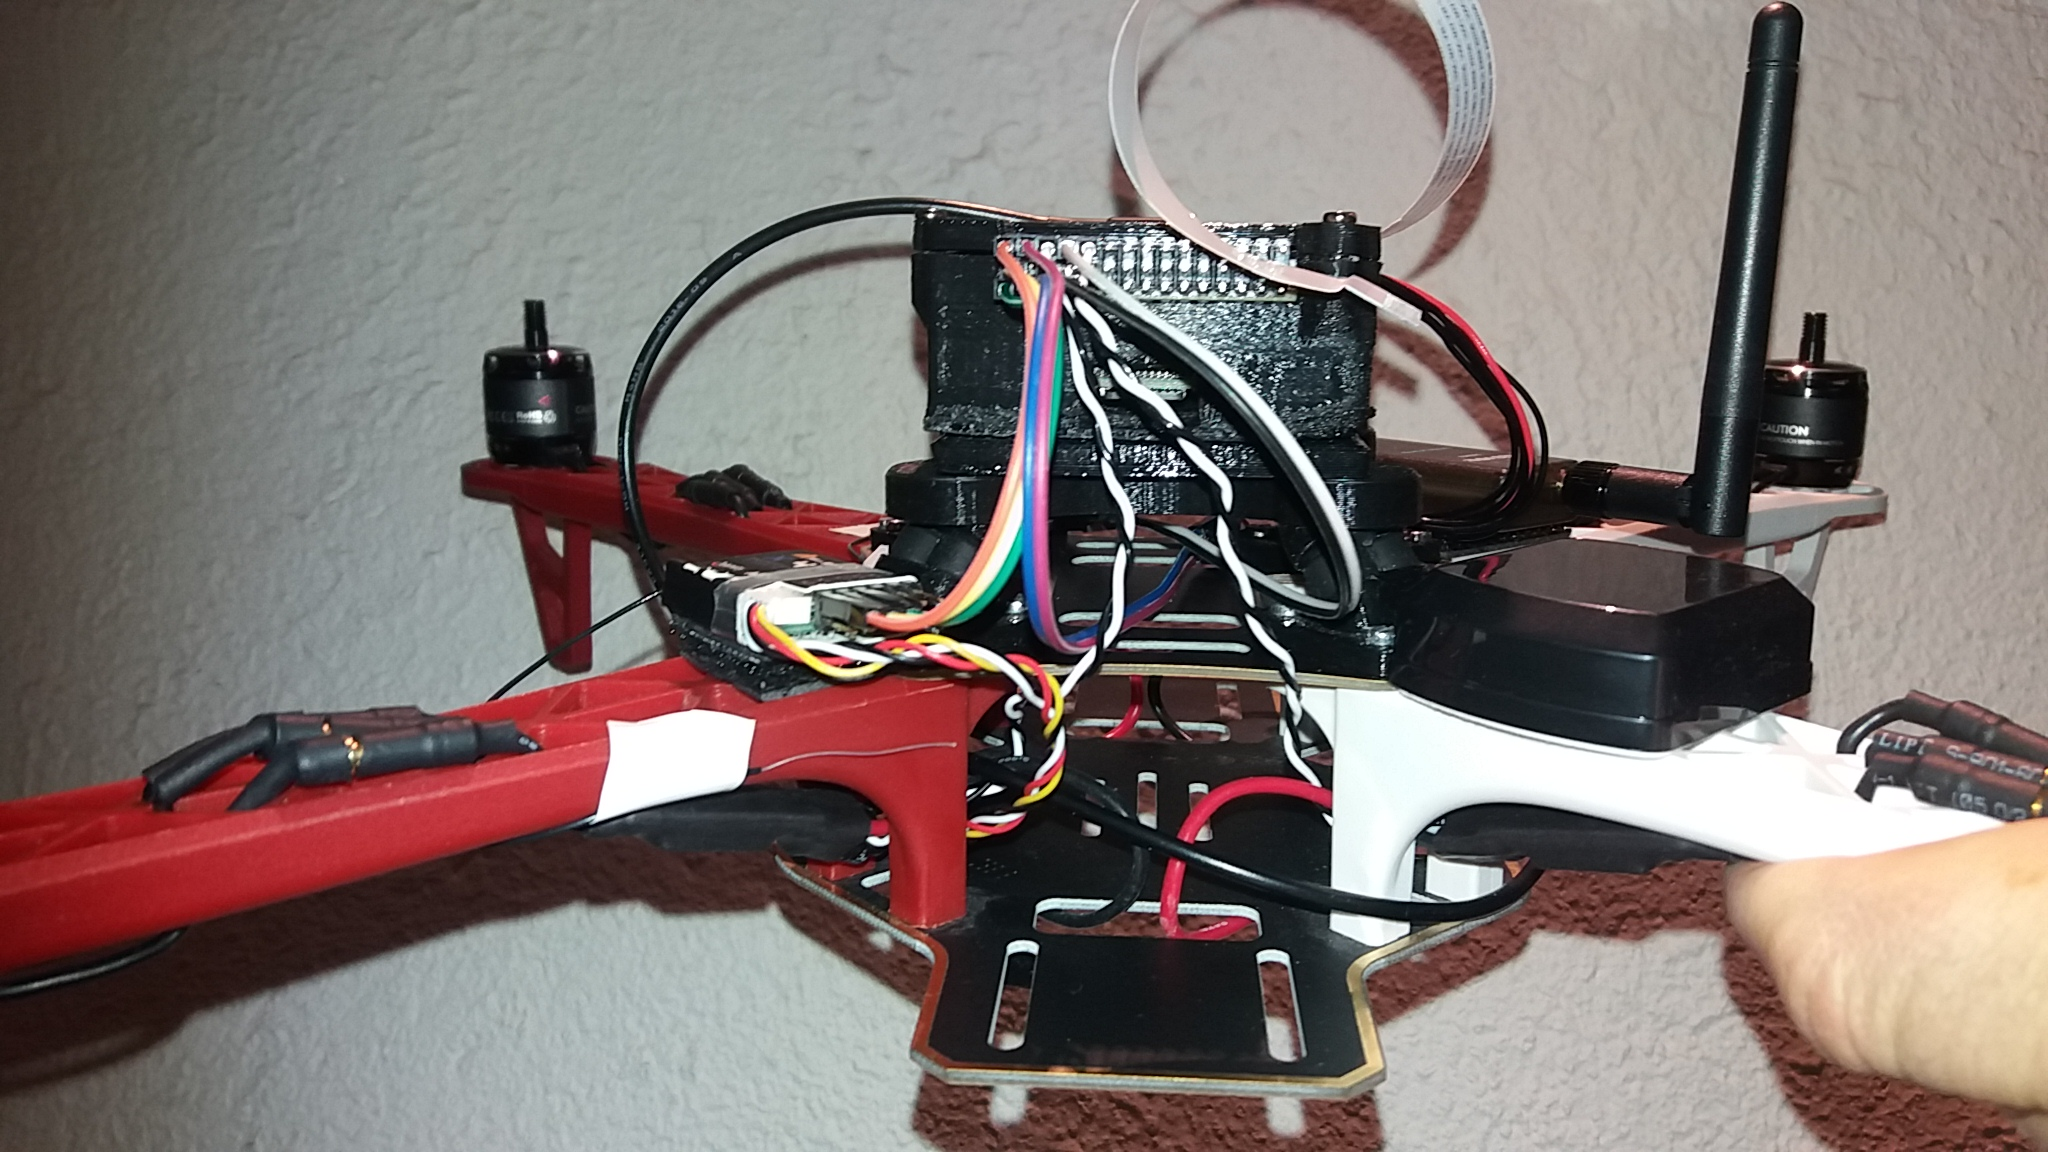
\includegraphics[scale=0.1]{images/drone-build-signal-wires.jpg}
\caption{Wiring up the signal wires}
\label{fig:attach_sbus}
\end{subfigure}
\begin{subfigure}{0.5\textwidth}
\centering
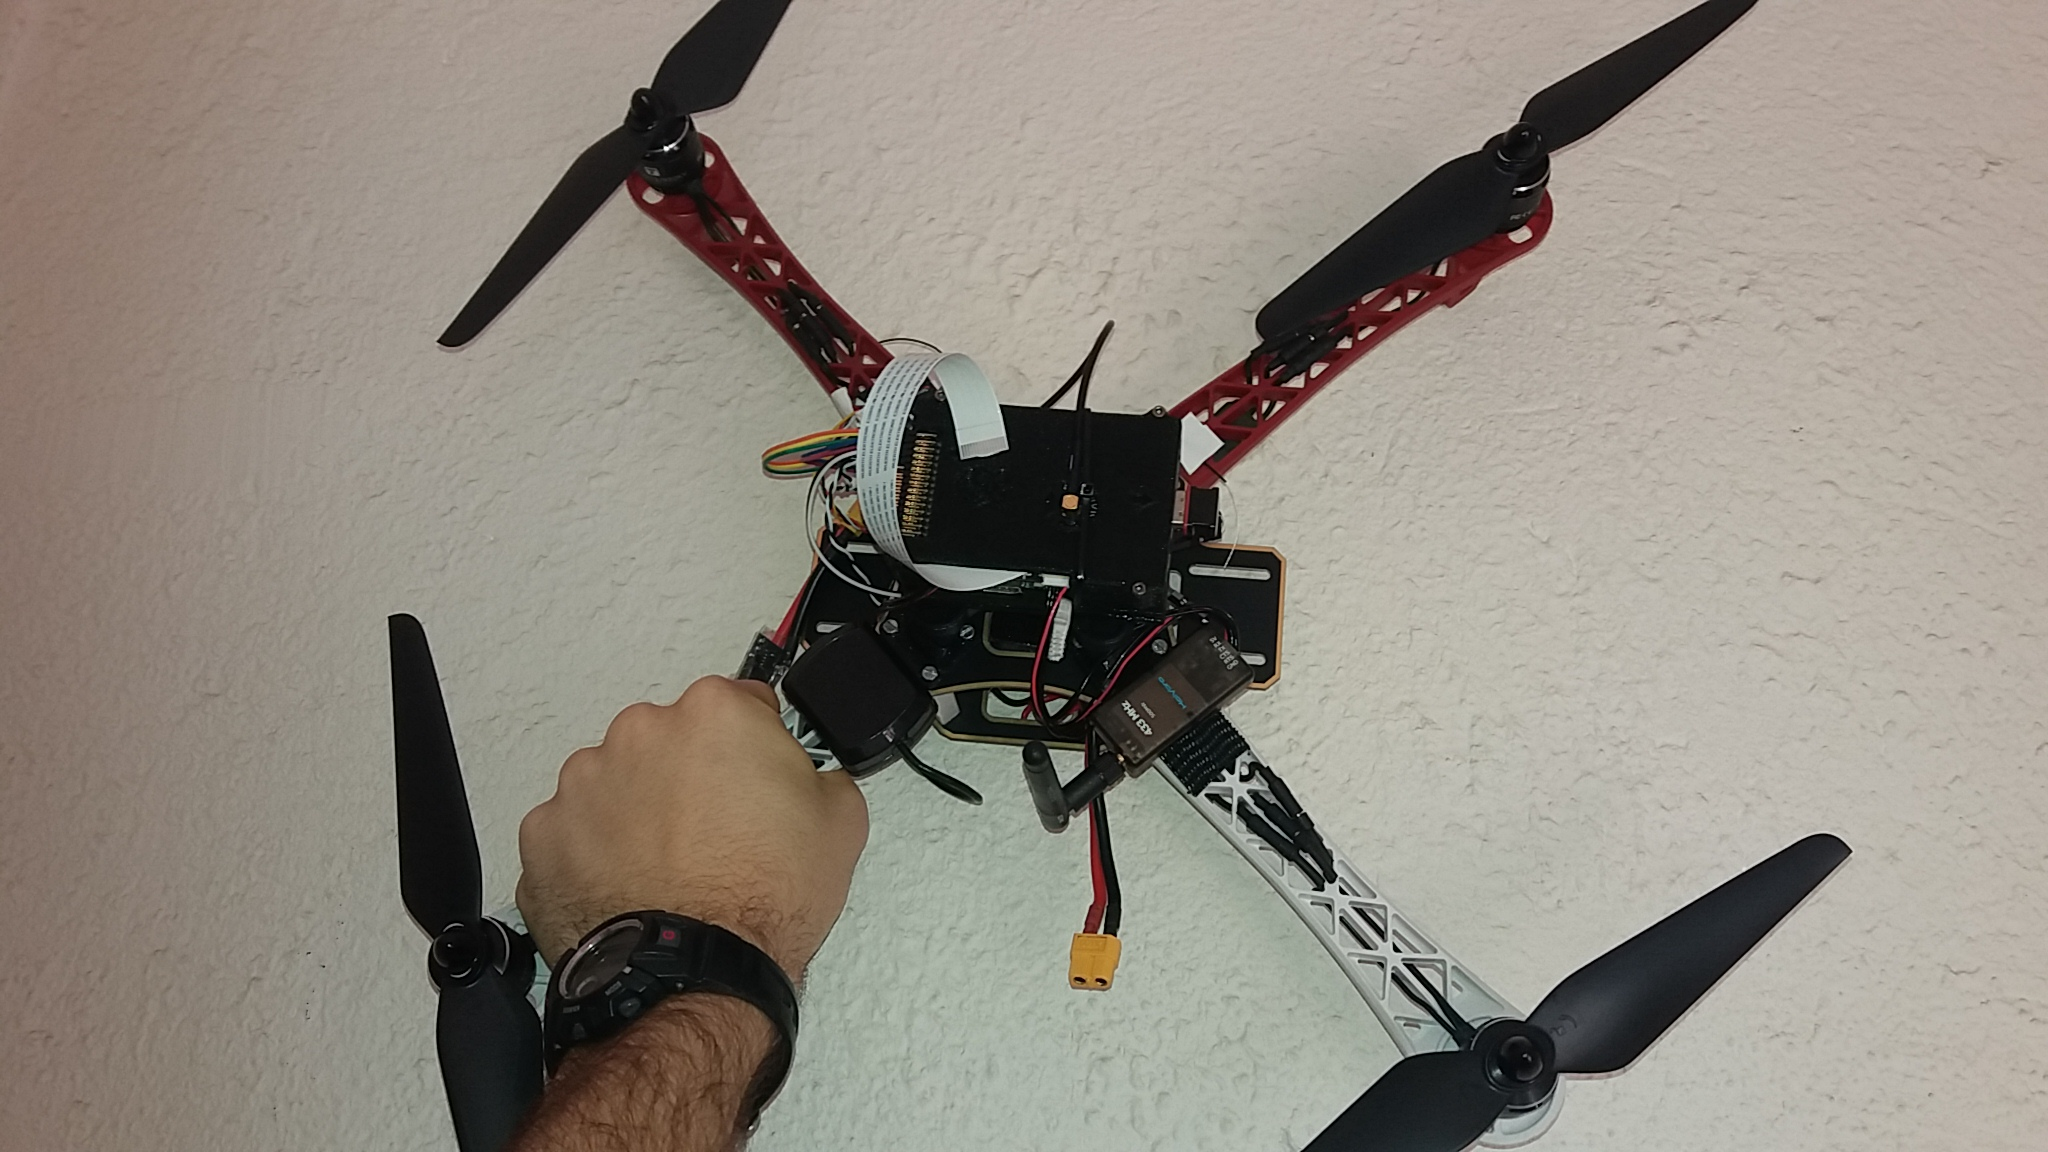
\includegraphics[scale=0.1]{images/drone-build-props.jpg}
\caption{Adding the 9.5'x4.5' propellers}
\label{fig:attach_props}
\end{subfigure}
\caption{Ready to fly}
\label{fig:attach_signal_props}
\end{figure}

The drone communicates with the handheld remote controller via S-BUS, which is a universal standard. The beauty of it is that it communicates with one signal wire as in Figure \ref{fig:attach_sbus}. Previous implementations one may have had to use pulse position modulation (PPM), where each channel requires a wire. Even though this may sound simple, it does increase PCB size, complexity and cost in the end.\\

One the other hand, each electronic speed controller (ESC) gets a signal wire and power input.

The propellers have a pitch of 4.5', which is basically a measure of the 'bite', or distance it travels through the air on one revolution.

\section{Ground Control Station}

An RF linkup (via an ISM band) with a GCS is necessary for pre-flight checks, and monitoring/controlling the status of the vehicle during flight.

The drone communicates with the GCS in Figure (picture of the GCS) using 433 MHz transceivers.

Show specs. Why? Pre-flight checks, setting waypoints.

(add a picture of the GCS).

The software used is the open source Mission Planner platform.

(insert MP picture).

\section{Remote controller}

Full-duplex remote controller returns battery and signal strength information, with the capability of sending other sensor data via SBUS.

(insert picture of remote controller).

Insert specs.

Set up steps.

\section{Software}

This will be handled by two Raspberry Pis. Both will be used to take photos through each of their single CSI ports. The Raspberry Pis will communicate with each other via direct ethernet connection. Twisted-pair is not necessary since the driver automatically swaps the RX and TX lines.

Initially, one Raspberry Pi was to be used with a camera multiplexer, but it didn't work, and therefore two raspberry pis were used. Just as well, as the flight controller uses all but 1 GPIO pin.

A real-time kernel will be used for the Ardupilot Firmware used on the flight controller Raspberry Pi.

\section{Testing}

Adjusting PID values.